\documentclass[spanish,a4paper,12pt,oneside]{extreport}

\usepackage[dvips]{graphicx}
\usepackage[dvips]{epsfig}
\usepackage[utf8]{inputenc}
\usepackage[spanish]{babel}
\usepackage{alltt}

\usepackage[ruled,vlined,commentsnumbered,linesnumbered,inoutnumbered,titlenotnumbered,noend]{algorithm2e}
\SetKwRepeat{Do}{do}{while}

\usepackage{multirow}
\usepackage{array} 
\usepackage{amsfonts}
\usepackage{amsmath}
\usepackage{bigstrut}
\usepackage{booktabs}
\usepackage{caption}
\usepackage{chngpage}
\usepackage{float}
\usepackage{enumitem,lipsum}
\usepackage{graphicx}
\usepackage{lscape}
\usepackage{microtype}
\usepackage{pdflscape}
\usepackage{rotating}
\usepackage{subcaption}
\usepackage{ctable}
\usepackage{hyperref}
\usepackage{enumerate}
\usepackage{gensymb}
\usepackage{eurosym}
\usepackage{xcolor}
\usepackage{tabu}

\usepackage{lineno}
%\\linenumbers
%\setlength\linenumbersep{5pt}
%\renewcommand\linenumberfont{\normalfont\tiny\sffamily\color{gray}}

\usepackage[top=2cm, bottom=2cm, left=2cm, right=2cm]{geometry}

\newenvironment{sourcecode}
{\begin{list}{}{\setlength{\leftmargin}{1em}}\item\scriptsize\bfseries}
{\end{list}}

\newenvironment{littlesourcecode}
{\begin{list}{}{\setlength{\leftmargin}{1em}}\item\tiny\bfseries}
{\end{list}}

\newenvironment{summary}
{\par\noindent\begin{center}\textbf{Abstract}\end{center}\begin{itshape}\par\noindent}
{\end{itshape}}

\newenvironment{keywords}
{\begin{list}{}{\setlength{\leftmargin}{1em}}\item[\hskip\labelsep \bfseries Keywords:]}
{\end{list}}

\newenvironment{palabrasClave}
{\begin{list}{}{\setlength{\leftmargin}{1em}}\item[\hskip\labelsep \bfseries Palabras clave:]}
{\end{list}}

\usepackage{bera}% optional: just to have a nice mono-spaced font
\usepackage{listings}
\usepackage{xcolor}

\colorlet{punct}{red!60!black}
\definecolor{background}{HTML}{EEEEEE}
\definecolor{delim}{RGB}{20,105,176}
\colorlet{numb}{magenta!60!black}

\lstdefinelanguage{json}{
    basicstyle=\normalfont\ttfamily,
    numbers=left,
    numberstyle=\scriptsize,
    stepnumber=1,
    numbersep=8pt,
    showstringspaces=false,
    breaklines=true,
    frame=lines,
    backgroundcolor=\color{background},
    literate=
     *{0}{{{\color{numb}0}}}{1}
      {1}{{{\color{numb}1}}}{1}
      {2}{{{\color{numb}2}}}{1}
      {3}{{{\color{numb}3}}}{1}
      {4}{{{\color{numb}4}}}{1}
      {5}{{{\color{numb}5}}}{1}
      {6}{{{\color{numb}6}}}{1}
      {7}{{{\color{numb}7}}}{1}
      {8}{{{\color{numb}8}}}{1}
      {9}{{{\color{numb}9}}}{1}
      {:}{{{\color{punct}{:}}}}{1}
      {,}{{{\color{punct}{,}}}}{1}
      {\{}{{{\color{delim}{\{}}}}{1}
      {\}}{{{\color{delim}{\}}}}}{1}
      {[}{{{\color{delim}{[}}}}{1}
      {]}{{{\color{delim}{]}}}}{1},
}

\begin{document}

\renewcommand\listtablename{Índice de Tablas}    
\renewcommand\listfigurename{Índice de Figuras}    

%%%%%%%%%%%%%%%%%%%%%%%%%%%%%%%%%%%%%%%%%%%%%%%%%%%%%%%%%%%%%%%%%%%%%%%%%%%%%%%
% First Page
%%%%%%%%%%%%%%%%%%%%%%%%%%%%%%%%%%%%%%%%%%%%%%%%%%%%%%%%%%%%%%%%%%%%%%%%%%%%%%%
\pagestyle{empty}
\thispagestyle{empty}


\newcommand{\HRule}{\rule{\linewidth}{1mm}}
\setlength{\parindent}{0mm}
\setlength{\parskip}{0mm}

\vspace*{\stretch{0.5}}

\begin{center}

\includegraphics[scale=0.8]{images/escuela-ingenieria-tecnologia-original}\\[10mm]
{\Huge Trabajo de Fin de Grado}
\end{center}

\HRule
\begin{flushright}
        {\Huge Titulo del trabajo} \\[2.5mm]
        {\Large \textit{Título del trabajo en inglés}} \\[5mm]
        {\Large Nombre y apellidos} \\[5mm]


\end{flushright}
\HRule
\vspace*{\stretch{2}}
\begin{center}
  \Large La Laguna, \today
\end{center}

\setlength{\parindent}{5mm}

%%%%%%%%%%%%%%%%%%%%%%%%%%%%%%%%%%%%%%%%%%%%%%%%%%%%%%%%%%
% Signature page (add the official stamp)
%%%%%%%%%%%%%%%%%%%%%%%%%%%%%%%%%%%%%%%%%%%%%%%%%%%%%%%%%%
\newpage
\thispagestyle{empty}

D. {\bf Nombre Apellido1 Apellido2}, con N.I.F. 12.345.678-X profesor Titular de Universidad adscrito al Departamento de Nombre del Departamento de la Universidad de La Laguna, como tutor

\bigskip
D. {\bf Nombre Apellido1 Apellido2}, con N.I.F. 12.345.678-X profesor Titular de Universidad adscrito al Departamento de Nombre del Departamento de la Universidad de La Laguna, como cotutor\pagestyle{empty}

\bigskip
\bigskip
{\bf C E R T I F I C A (N)}

\bigskip
\bigskip
Que la presente memoria titulada:

\bigskip
''{\it Título del Trabajo}''

\bigskip
\bigskip
\bigskip

\noindent ha sido realizada bajo su dirección por D. {\bf Nombre Apellido1 Apellido2},
con N.I.F. 12.345.678-X.

\bigskip
\bigskip

Y para que así conste, en cumplimiento de la legislación vigente y a los efectos
oportunos firman la presente en La Laguna a \today

%%%%%%%%%%%%%%%%%%%%%%%%%%%%%%%%%%%%%%%%%%%%%%%%%%%%%%%%%%
\newpage
\thispagestyle{empty}

{ \flushright

\begin{LARGE}
Agradecimientos
\end{LARGE}

\hspace{3mm}

\begin{large}
XXXXX
\end{large}

}
%%%%%%%%%%%%%%%%%%%%%%%%%%%%%%%%%%%%%%%%%%%%%%%%%%%%%%%%
\newpage
\thispagestyle{empty}

\bigskip
\begin{LARGE}
Licencia
\end{LARGE}

\bigskip
* Si NO quiere permitir que se compartan las adaptaciones de tu obra y NO quieres permitir usos comerciales de tu obra indica:

\begin{center}

\includegraphics[scale=1.8]{images/by-nc-nd_88x31}\\[5mm]
\end{center}

\begin{large}
© Esta obra está bajo una licencia de Creative Commons Reconocimiento-NoComercial-SinObraDerivada 4.0 Internacional.
\end{large}

\bigskip
\bigskip
\bigskip
* Si quiere permitir que se compartan las adaptaciones de tu obra mientras se comparta de la misma manera y NO quieres permitir usos comerciales de tu obra indica:

\begin{center}

\includegraphics[scale=1.8]{images/by-nc-sa_88x31}\\[5mm]
\end{center}

\begin{large}
© Esta obra está bajo una licencia de Creative Commons Reconocimiento-NoComercial-CompartirIgual 4.0 Internacional.
\end{large}

\bigskip
\bigskip
\bigskip
* Si quiere permitir que se compartan las adaptaciones de tu obra y NO quieres permitir usos comerciales de tu obra indica:

\begin{center}

\includegraphics[scale=1.8]{images/by-nc_88x31}\\[5mm]
\end{center}

\begin{large}
© Esta obra está bajo una licencia de Creative Commons Reconocimiento-NoComercial 4.0 Internacional.
\end{large}

%%%%%%%%%%%%%%%%%%%%%%%%%%%%%%%%%%%%%%%%%%%%%%%%%%%%%%%%
\newpage
\thispagestyle{empty}

\bigskip
*Si NO quiere permitir que se compartan las adaptaciones de tu obra y quieres permitir usos comerciales de tu obra indica:

\begin{center}

\includegraphics[scale=1.8]{images/by-nd_88x31}\\[5mm]
\end{center}

\begin{large}
© Esta obra está bajo una licencia de Creative Commons Reconocimiento-SinObraDerivada 4.0 Internacional.
\end{large}

\bigskip
\bigskip
\bigskip
* Si quiere permitir que se compartan las adaptaciones de tu obra mientras se comparta de la misma manera y quieres permitir usos comerciales de tu obra (licencia de Cultura Libre) indica:

\begin{center}

\includegraphics[scale=1.8]{images/by-sa_88x31}\\[5mm]
\end{center}

\begin{large}
© Esta obra está bajo una licencia de Creative Commons Reconocimiento-CompartirIgual 4.0 Internacional.
\end{large}

\bigskip
\bigskip
\bigskip
* Si quiere permitir que se compartan las adaptaciones de tu obra y quieres permitir usos comerciales de tu obra (licencia de Cultura Libre) indica:

\begin{center}

\includegraphics[scale=1.8]{images/by_88x31}\\[5mm]
\end{center}

\begin{large}
© Esta obra está bajo una licencia de Creative Commons Reconocimiento 4.0 Internacional.
\end{large}

%%%%%%%%%%%%%%%%%%%%%%%%%%%%%%%%%%%%%%%%%%%%%%%%%%%%%%%%
\newpage 
\thispagestyle{empty}

\begin{abstract}
{\em
xxxxx
}

\begin{palabrasClave}
xxxxx, xxxx, xxxx
\end{palabrasClave}

\end{abstract}
%%%%%%%%%%%%%%%%%%%%%%%%%%%%%%%%%%%%%%%%%%%%%%%%%%%%%%%%%
\newpage 
\vspace*{200px}
\thispagestyle{empty}

\begin{summary}
{
xxxxx
}

\em
\begin {keywords}
xxxx, xxxx, xxxx
\end {keywords}

\end{summary}
%%%%%%%%%%%%%%%%%%%%%%%%%%%%%%%%%%%%%%%%%%%%%%%%%%%%%%%%%
\newpage{\pagestyle{empty}}
\thispagestyle{empty}

%%%%%%%%%%%%%%%%%%%%%%%%%%%%%%%%%%%%%%%%%%%%%%%%%%%%%%%%%
\pagestyle{myheadings} %my head defined by markboth or markright
% No funciona bien \markboth sin "twoside" en \documentclass, pero al
% ponerlo se dan un montón de errores de underfull \vbox, con lo que no se
% ha puesto.


%%Aqui debería poner el nombre del proyecto pero, como es muy grande no cabe y se ve feo en el PDF
\markboth{xxxxx}{}

%%%%%%%%%%%%%%%%%%%%%%%%%%%%%%%%%%%%%%%%%%%%%%%%%%%%%%%%%
%Numeracion en romanos
\renewcommand{\thepage}{\roman{page}}
\setcounter{page}{1}
\pagestyle{plain} 

%%%%%%%%%%%%%%%%%%%%%%%%%%%%%%%%%%%%%%%%%%%%%%%%%%%%%%%%%

\tableofcontents

%%%%%%%%%%%%%%%%%%%%%%%%%%%%%%%%%%%%%%%%%%%%%%%%%%%%%%%%%
\newpage{\pagestyle{empty}}

\listoffigures

%%%%%%%%%%%%%%%%%%%%%%%%%%%%%%%%%%%%%%%%%%%%%%%%%%%%%%%%%
\newpage{\pagestyle{empty}}

\listoftables

%%%%%%%%%%%%%%%%%%%%%%%%%%%%%%%%%%%%%%%%%%%%%%%%%%%%%%%%%%%%%%%%%%%%%%%%%%%%%%%
\newpage{\pagestyle{empty}}

%%%%%%%%%%%%%%%%%%%%%%%%%%%%%%%%%%%%%%%%%%%%%%%%%%%%%%%%%%%%%%%%%%%%%%%%%%%%%%%
\newpage
\thispagestyle{empty}

%Numeracion a partir del capitulo I
\renewcommand{\thepage}{\arabic{page}}
\setcounter{page}{1}
\pagestyle{plain}

\chapter{\LARGE Introducción}
\label{chapter:intro}

\section{Computación de altas prestaciones}
\vspace{2mm}
La computación de altas prestaciones (HPC, High Performance Computing por sus siglas en inglés) es una forma de procesar grandes volúmenes de datos a velocidades muy altas utilizando varios ordenadores y dispositivos de almacenamiento \cite{hpccomputing}. Este campo nace de la necesidad de resolver problemas computacionales muy complejos, generalmente de la ciencia y de la ingeniería. 
\vspace{2mm}

\vspace{2mm}
Numerosas son las aplicaciones que tiene \cite{hpcexamples} y los beneficios que aporta a los ciudadanos, a la industria y a la ciencia \cite{benefitscomputing}.
\vspace{4mm}

En los beneficios para los ciudadanos, la supercomputación es clave para el avance de la medicina: permite descubrir nuevos medicamentos, desarrollar terapias médicas que cubran necesidades individuales y estudiar enfermedades genéticas poco comunes. Ha permitido en la actualidad desarrollar los tratamientos para el COVID-19. Adicionalmente, permite monitorizar los efectos del cambio climático así como mejorar nuestro conocimiento de los procesos geofísicos y realizar simulaciones que predigan la evolución del tiempo a partir de sus patrones.

\vspace{2mm}
Para la industria (automóvil, aeroespacial, energías renovables), los supercomputadores permiten innovar, ser más productivos y escalar con productos de mayor valor y servicio, reduciendo los ciclos de diseño y producción y acelerando el diseño de nuevos materiales, gracias a que minimiza los costes, incrementa la eficiencia de recursos y acorta y optimiza los procesos de decisión.
\vspace{2mm}

Por último, en la ciencia, permite avanzar los conocimientos que tenemos sobre la materia y explorar el universo, así como modelar la atmósfera y el fenómeno oceánico a nivel planetario.
\vspace{4mm}

Un ejemplo de sistema de computación de altas prestaciones existentes podría ser el Teide-HPC \cite{teidehpc}, perteneciente al ITER (Instituto Tecnológico y de Energías Renovables) y que se encuentra en Tenerife. Está compuesto por 1100 servidores de cómputo Fujitsu, con un total de 17800 cores de cómputo y 36 TB de memoria, siendo así el segundo más potente de España y, hasta el 2015, uno de los top 500 supercomputadores más potentes del mundo \cite{teidehpcranking}.
\vspace{2mm}

En España se ubica también el supercomputador Marenostrum \cite{marenostrum}, que es considerado el sexagésimo tercer computador más potente del mundo en la última revisión de junio de 2021 \cite{marenostrumtop}. La última versión del Marenostrum tiene un rendimiento pico de 13.9 flops y se compone de dos bloques: uno de propósito general, que tiene 165.888 procesadores en total y una memoria central de 390 terabytes, y otro de tecnologías emergentes, que está formado por tres clusters de tecnologías que se están desarrollando actualmente en Estados Unidos y Japón para la nueva generación de supercomputadores pre-exascala.

\vspace{2mm}

A nivel Europeo, el sector de la computación de altas prestaciones no para de crecer. Actualmente, existe la iniciativa Eurohpc \cite{eurohpc} que, con un presupuesto de mil millones de euros, se están construyendo 7 supercomputadores en toda Europa,  se espera que dos de ellos estén dentro del top 5 mundial: LUMI, localizado en Finlandia, con un rendimiento máximo de 552 petaflops y Leonardo, en Italia, con un rendimiento máximo de 322.6 petaflops.


\vspace{4mm}
En la computación de altas prestaciones no importa únicamente la cantidad de núcleos y la potencia que tiene el hardware, sino que también debe tenerse en cuenta cómo se desarrolla el software que va a ejecutarse sobre la máquina, para maximizar el rendimiento. Para ello, se emplea la programación paralela.

\section{Programación paralela}

La programación paralela es una técnica en la que muchas instrucciones se ejecutan de forma simultánea. Se basa en el principio de "Divide y vencerás": los problemas grandes se pueden dividir en partes más pequeñas que pueden resolverse de forma concurrente. 
\vspace{2mm}
Existen varios tipos de computación paralela \cite{tiposparalelismo}:
\vspace{2mm}
\begin{itemize}
    \item \textbf{Paralelismo a nivel de bit: } cuando se aumenta el tamaño de la palabra del procesador, se habla de paralelismo a nivel de bit.
    \vspace{2mm}

    Por ejemplo, al operar con dos números de 16 bits sobre un procesador de 8 bits, se requeriría de dos instrucciones, mientras que si el procesador fuera de 16 bits, esta se podría realizar en una sola instrucción.
    
    \item \textbf{Paralelismo a nivel de instrucción: } consiste en cambiar el orden de las instrucciones de un programa y juntarlas en grupos, siempre sin alterar el resultado final del programa.
    \vspace{2mm}

    Esto se puede hacer gracias a que los procesadores modernos tienen N etapas por los que pasan las instrucciones, por lo que ese procesador puede ejecutar hasta N instrucciones diferentes simultáneamente con la ordenación y agrupación adecuada.

    \item \textbf{Paralelismo de datos: } cada procesador realiza la misma tarea sobre un subconjunto independiente de datos. 
    
    Es muy común utilizarlo en big data, especialmente cuando se opera con una gran cantidad de datos que no es posible cargar en memoria.
    
    \item \textbf{Paralelismo de tareas: } cada hilo realiza una tarea distinta e independiente al resto.
    
    Un ejemplo podría ser una aplicación de mensajería instantánea, donde un hilo se encuentra pendiente para recibir información y otro está pendiente para la entrada de texto del cliente.
\end{itemize}
\vspace{2mm}

En los últimos años, el interés por la computación paralela aplicada en la computación de altas prestaciones ha aumentado debido a las restricciones físicas que impiden el escalado en frecuencia del hardware. Los ordenadores paralelos se pueden clasificar según el nivel de paralelismo que admite su hardware \cite{parallelcomputers}:
\vspace{2mm}

\begin{itemize}
    \item \textbf{Procesamiento multinúcleo.} La máquina tiene más de una unidad de CPU, por lo que puede procesar múltiples instrucciones por ciclo de secuencias. Si el núcleo es superescalar, adicionalmente, en cada ciclo puede ejecutar múltiples instrucciones de un flujo de instrucciones.
    \item \textbf{Multiprocesamiento simétrico.} Se trata de un sistema computacional con múltiples procesadores iguales que comparten memoria y están conectados a través de un bus.
    \item \textbf{Computación en cluster.} Se trata de un grupo de ordenadores independientes que trabajan en colaboración por red. El más típico es el cluster Beowulf \cite{beowulf}, que implementa múltiples ordenadores idénticos conectados a una red local por Ethernet.
    \item \textbf{Computación distribuida. } Se hace uso de ordenadores que se comunican a través de Internet para trabajar en un problema dado. Normalmente, se refiere a problemas vergonzosamente paralelos, ya que la latencia es demasiado alta y el ancha de banda es bajo.
\end{itemize}

\vspace{2mm}
Los dos paradigmas principales de la programación paralela son el paso de mensajes y la memoria compartida \cite{paradigmasparalelismo}.
\vspace{2mm}

El paradigma de paso de mensajes es ampliamente utilizado en el software moderno para ejecutar tareas sincronizadas entre varios ordenadores.

\vspace{2mm}
Para ello, se intercambia información de forma síncrona o asíncrona. La manera síncrona es sencilla de implementar, pero su inconveniente es que es poco flexible, ya que bloquea el proceso hasta que se realiza el intercambio de mensajes entre procesos. El intercambio de mensajes de forma asíncrona no produce bloqueos en el código, sin embargo, puede generar fallos de seguridad cuando se intercambian y manipulan variables.

\vspace{2mm}
En el paradigma de memoria compartida, el intercambio de datos entre programas se realiza reservando un área de RAM en la que otro proceso puede acceder. Así, cuando se modifiquen valores dentro de este área, será visible para los demás procesos.

\vspace{2mm}
El desarrollo de programas informáticos paralelos es más complejo que los secuenciales. 
\vspace{2mm}

La concurrencia introduce nuevos tipos de errores de software, como las condiciones de carrera y añade nuevos problemas como la sincronización entre diferentes subtareas. 
\vspace{2mm}


Además, no todas las paralelizaciones conllevan una aceleración. Generalmente, mientras una tarea se divida en cada vez más hilos, estos hilos pasan una porción cada vez mayor de su tiempo comunicándose entre sí. Eventualmente, la sobrecarga de comunicación domina el tiempo empleado para resolver el problema, y la paralelización adicional aumenta la cantidad de tiempo requerido para terminar.
\vspace{2mm}


%%%%%%%%%%%%%%%%%%%%%%%%%%%%%%%%%%%%%%%%%%%%%%%%%%%%%%%%%%%%%%%%%%%%%%%%%%%%%%%
\newpage{\pagestyle{empty}}
\thispagestyle{empty}

\chapter{\LARGE Título del Capítulo 2}
\label{chapter:dos}

En este capítulo se describe el estado del arte tanto antes de empezar el proyecto como después, así como los recursos disponibles, el análisis de posibles herramientas y las herramientas utilizadas para llevar a cabo la configuración del \emph{cluster} para computación de altas prestaciones.

\section{Estado del arte}

Antes de comenzar el proyecto, el grupo de investigación PAL (Parallel Algorithms and Languages) contaba ya con tres máquinas con las que realizar computación de altas prestaciones: Bolido, Rayo y Centella.
\vspace{2mm}

Cada una de estas máquinas tiene un procesador AMD con 48 núcleos y 64 gigas de RAM. Bolido tiene dos discos duros de 500GB: uno de tipo SAS y otro SATA. Rayo también cuenta con dos discos duros, aunque ambos son de tipo SAS y Centella cuenta con un único disco duro de 500GB de tipo SAS.
\vspace{2mm}

Estas máquinas se utilizaban de manera individual y no tenían ningún mantenimiento ni ninguna gestión. Los usuarios accedían a cualquiera de ellas cuando necesitaban realizar alguna prueba, compilaban su código y lo dejaban ejecutándose con un número de procesadores determinados. Con el paso de los años, el sistema operativo de estas máquinas quedó también obsoleto.
\vspace{2mm}
 
Con el afán de poner en funcionamiento de nuevo estas máquinas y organizar mejor los recursos disponibles, se decidió actualizar y configurar de nuevo los sistemas y crear un cluster, en el que se centralicen los usuarios y la gestión de las máquinas disponibles.
\vspace{2mm}

Para la actualización de los sistemas, se tuvo que ir físicamente al STIC (Servicio TIC de la Universidad de La Laguna) porque la interfaz remota iDRAC \cite{idrac} del servidor era demasiado lenta. En concreto, Bolido y Centella se tuvieron que instalar desde cero, para configurar el sistema con LVM (gestor de volúmenes lógicos) y Debian 10.
\vspace{2mm}

Por último, se realizó la configuración del cluster con distintas herramientas open source y se realizó un análisis de rendimiento.
\vspace{2mm}

\section{Buenas prácticas}

Es conveniente que al implementar un \emph{cluster} se utilicen una serie de buenas prácticas, con el fin de facilitar tanto el mantenimiento como la administración del sistema en el futuro y mantener seguros los sistemas. Para este caso, me he apoyado en un paper sobre las mejores prácticas antes de implementar el sistema \cite{6114480} y de elegir las herramientas.
\vspace{2mm}

Para nuestro caso, lo que más nos interesa en nuestro sistema es minimizar el trabajo de administración y gestión de sistemas. Esto lo logramos con:

\begin{itemize}
    \item \textbf{Centralización: } conviene que todo lo que sea común en todas las máquinas se encuentre centralizado: usuarios, librerías, software, autenticación, manejo de recursos.
    \item \textbf{Escalabilidad: } hacer que las modificaciones del \emph{cluster} sean lo más sencillas posibles, tanto para añadir como para eliminar nodos. 
    \item \textbf{Administración de sistemas mínimo: } trazabilidad sencilla y sistemas robustos. Administrar muchas máquinas puede ser complejo, por lo que es conveniente que los sistemas sean lo más minimalistas posibles, especialmente los nodos.
    \item \textbf{Administración flexible del entorno de usuario: } permitir al usuario modificar el entorno de software fácilmente y ajustarlo a sus necesidades.
\end{itemize}



\section{Análisis de herramientas}

Existen diversas herramientas para configurar un \emph{cluster} para realizar programación paralela. En este apartado, se definen las herramientas utilizadas para la implementación de nuestro sistema y las alternativas que se han encontrado y descartado.

\subsection{Slurm}

Para el sistema HPC, necesitábamos un software que permitiera aceptar trabajos, planificarlos y monitorizarlos. Básicamente, un software de planificación de tareas. Para ello, se decidió utilizar Slurm \cite{slurmquickstart}.
\vspace{2mm}

Slurm es un planificador de tareas de código abierto \cite{slurmrepo} para sistemas basados en Linux que es tolerable a fallos y que permite escalar la gestión de sistemas distribuidos.
\vspace{2mm}

Con Slurm, se puede asignar usuarios a nodos de cómputo, con acceso no exclusivo, exclusivo, con recursos compartidos o con recursos limitados. Permite también iniciar, realizar y monitorizar los trabajos sobre los nodos y gestionar las colas de trabajos pendientes.
\vspace{2mm}

Adicionalmente, se puede extender con diferentes plugins, para realizar autenticación, registro de tareas completadas, gestión de energía, etc.
\vspace{2mm}

Como alternativa, se consideró TORQUE y Kubernetes.

\vspace{2mm}
TORQUE (Terascale Open-source Resource and Queue manager) \cite{torquerepo} es un planificador de trabajos similar a Slurm que no llegó a mantenerse en el tiempo, por lo que no era conveniente utilizarlo.

\vspace{2mm}
Kubernetes \cite{kubernetesrepo} es un orquestador de código abierto para cargas de trabajo basadas en contenedores. Permite manejar cargas de trabajo similar a un cluster HPC, aunque no ofrece todas las capacidades de gestión de trabajos que slurm. 

\vspace{2mm}
Kubernetes se basa en cluster de nodos que se controlan por un master. Cada nodo tiene una serie de contenedores que comparten recursos y existen en la red local, por lo que pueden comunicarse entre sí. Se descartó debido a que su uso es idóneo para escalar tecnologías \emph{cloud} y contenedores basados en microservicios, mientras que slurm permite lanzar aplicaciones en escala.

\subsection{Munge}

Munge \cite{munge} es un servicio de autenticación para crear y validar credenciales, diseñado para ser escalable en sistemas distribuidos.
\vspace{2mm}

Es un software completamente necesario para el funcionamiento correcto de slurm, ya que lo utiliza para autenticar los trabajos.

\subsection{OpenSSH}

Para la conexión remota cifrada entre máquinas, se utilizó OpenSSH \cite{openssh}, que es la implementación libre utilizada generalmente en sistemas linux.

\subsection{OpenLDAP}

Para el acceso unificado a la información de red y autenticación centralizada, se utilizó OpenLDAP \cite{openldap}.

\vspace{2mm}

En concreto, se comparten en todos los sistemas los ficheros /etc/passwd y /etc/group globales para la autenticación de los usuarios.

\subsection{NTP}

Se utiliza la implementación de NTP para sincronizar los relojes del cluster, completamente necesario para evitar problemas
\vspace{2mm}

Como alternativa, existe chrony \cite{chrony}. 
\vspace{2mm}

Para nuestro caso de uso, es preferible utilizar el demonio NTP porque nuestros sistemas siempre están conectados por red. Chrony se considera mejor para sistemas que se desconectan de una red o se suspenden de forma frecuente, ya que tiene una sincronización más rápida y mejor respuesta a los cambios en la frecuencia del reloj \cite{chronyvsntp}.

\subsection{NFS}

Por último, se utilizó NFS \cite{nfs} (Network File System) para centralizar el software disponible y las carpetas de los usuarios. En cambio, autofs  \cite{nfsautofs} se utilizó para montar dichos directorios en los clientes (nodos de cómputo).



%%%%%%%%%%%%%%%%%%%%%%%%%%%%%%%%%%%%%%%%%%%%%%%%%%%%%%%%%%%%%%%%%%%%%%%%%%%%%%%
\newpage{\pagestyle{empty}}
\thispagestyle{empty}

\chapter{\LARGE Título del Capítulo 3}
\label{chapter:tres}

Los capítulos intermedios servirán para cubrir los siguientes aspectos: antecedentes, problemática o estado del arte, objetivos, fases y desarrollo del proyecto.

\bigskip
Bla, Bla, Bla, .....

\section{Primera sección de este capítulo}
\section{Segundo apartado de este capítulo}
\section{Tercer apartado de este capítulo}

%%%%%%%%%%%%%%%%%%%%%%%%%%%%%%%%%%%%%%%%%%%%%%%%%%%%%%%%%
\newpage{\pagestyle{empty}}
\thispagestyle{empty}

\chapter{\LARGE Título del Capítulo 4}
\label{chapter:cuatro}

\section{Análisis del rendimiento}

Tras configurar el cluster,  se realizaron algunos experimentos con el fin de comprobar el funcionamiento correcto y realizar un análisis del rendimiento de las máquinas.

Para hacer pruebas, se utilizó un programa sencillo que calcula el valor de pi encontrado en un repositorio de github \cite{openmpirepo}. Este programa se utilizó simplemente para comprobar que todo funcionaba y familiarizarse con slurm. 

Después, para realizar un análisis de rendimiento, se utilizó NPB: un \emph{benchmark} perteneciente a la NASA, interesante especialmente porque las distintas pruebas de paralelización utilizan la memoria de distintas formas.

\subsection{Métricas}

El objetivo principal del análisis de rendimiento es conseguir los mejores resultados en el menor tiempo posible y consumiendo el menor número de recursos posible.
\vspace{2mm}

A la hora de determinar el rendimiento de una arquitectura paralela, es común medir la eficiencia mediante estas dos medidas \cite{parelismoyrendimiento}:
\vspace{2mm}

\begin{itemize}
\item \textbf{Tiempo de ejecución o respuesta} de una aplicación.

\item \textbf{Productividad} (\emph{throughput}), el número de aplicaciones que es capaz de procesar por unidad de tiempo.
\end{itemize}

\vspace{2mm}
Sin embargo, aunque ofrecen información útil, son medidas demasiado simples, por lo que se introducen otras métricas como el \emph{speedup}, la eficiencia, la utilización, la redundancia y la calidad del paralelismo.

\vspace{6mm}
\textbf{Aceleración}
\vspace{2mm}

El \emph{speedup} mide la relación entre el tiempo de ejecución de un algoritmo en paralelo con respecto a lo que tarda el mismo algoritmo en resolver el problema de forma secuencial.

\begin{equation*}
    S(n) = \frac{T(1)}{T(n)}
\end{equation*}

Generalmente, speedup tiene un valor entre 0 y p (número de procesadores), donde lo ideal sería que fuera igual a p (Figura \ref{speedup}). Sin embargo, también cabe la posibilidad que el valor sea mayor que p, causando así un speedup superlineal. Cuando esto ocurre, suele deberse a la gestión interna de la memoria en el caso del algoritmo paralelo, en el que cada procesador trabaja con menos datos que en el algoritmo secuencial.
\vspace{4mm}

\begin{figure}[htb]
   \centering
   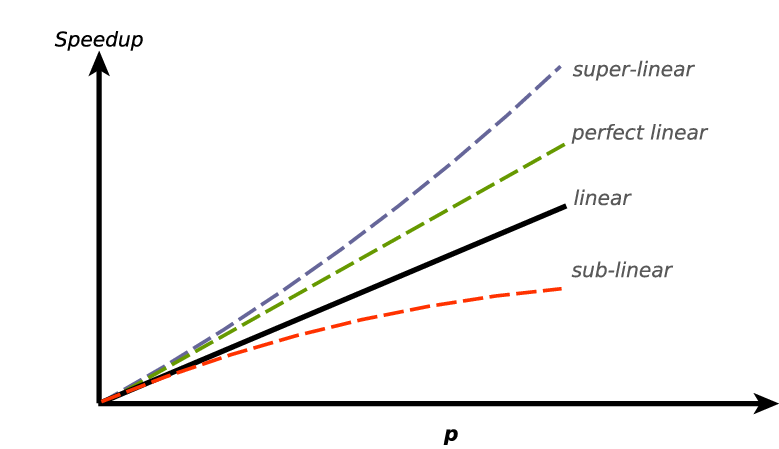
\includegraphics[scale=0.3]{images/speedup.png}
   \caption{SpeedUp}
   \label{speedup}
\end{figure}

\vspace{4mm}
\textbf{Eficiencia}
\vspace{2mm}

La eficiencia mide la fracción de tiempo durante la cual se utiliza de manera útil un procesador. Se obtiene dividiendo el speedup entre el número de procesadores.

\vspace{2mm}
\begin{equation*}
    E(n) = \frac{S(n)}{n} = \frac{T(1)}{n*T(n)}
\end{equation*}
\vspace{2mm}

Esta medida tendrá un valor entre 0 y 1, siendo 1 el valor ideal. Como ocurre con el speedup, también podemos obtener una eficiencia superior, si el speedup es superlineal.

\vspace{4mm}
\textbf{Redundancia}
\vspace{2mm}

La redundancia en un cálculo paralelo se define como el número total de operaciones ejecutadas con n procesadores dividido por el número de operaciones ejecutadas cuando utilizamos un único procesador.

\begin{equation*}
    R(n) = \frac{O(n)}{O(1)}
\end{equation*}

\vspace{4mm}
\textbf{Utilización}
\vspace{2mm}

La utilización de un sistema indica el porcentaje de recursos que se utilizan durante la ejecución de un programa paralelo.

\begin{equation*}
    U(n) = R(n)E(n) = \frac{O(n)}{n * T(n)}
\end{equation*}


\vspace{4mm}
\textbf{Calidad del paralelismo}
\vspace{2mm}

La calidad de un cálculo paralelo es directamente proporcional al speedup y la eficiencia, inversamente proporcional a la redundancia.
\vspace{2mm}

\begin{equation*}
    Q(n) = \frac{S(n)*E(n)}{R(n)} = \frac{T^{3}(1)}{n*T^{2}(n)*O(n)}
\end{equation*}
\vspace{2mm}

Al combinar el speedup, la eficiencia y la redundancia en una expresión, con la calidad medimos el mérito relativo de un cálculo paralelo en un sistema.

\section{Cálculo de PI}

Se utilizó un programa de ejemplo del calculo de PI con OpenMPI de un repositorio de Github \cite{piprogram} para hacer pruebas rápidas y ver que el cluster se encontraba funcionando correctamente. Fue especialmente útil para interactuar con el sistema como si fuera un usuario para detectar errores y aspectos a mejorar, así como familiarizarse con slurm y comprender su funcionamiento.
\vspace{2mm}

Por ejemplo, con los siguientes comandos, se carga el modulo de OpenMPI, se reservan 16 CPUs de los 2 nodos que hay en el sistema y se lanza un trabajo que ejecutará el cálculo de Pi.

\vspace{2mm}
\begin{lstlisting}[language=bash]
    $ module load openmpi
    $ salloc -N 2 -n 16
    $ srun -N 2 -n 16 --mpi=pmi2 ./pi
\end{lstlisting}
\vspace{2mm}

\section{NAS Parallel Benchmarks}
NAS Parallel Benchmarks (NPB) es un conjunto de programas que fueron diseñados para evaluar el rendimiento de ordenadores paralelos \cite{nasbenchmark}. El banco de pruebas está compuesto distintos tipos de pruebas:

\begin{itemize}
    \item \textbf{IS: } Integer Sort, acceso aleatorio a memoria.
    \item \textbf{EP: } Embarrassingly Parallel: problemas en los que no hay apenas dificultades en separarlos en tareas paralelas.
    \item \textbf{CG:} Conjugado del gradiente. Acceso irregular a memoria.
    \item \textbf{MG: } Multi Grid en una secuencia de mallas. Utiliza memoria de forma intensiva.
    \item \textbf{FT: } transformada de Fourier en 3 dimensiones. Intensivo en comunicaciones
    \item \textbf{BT:} Resuelve matrices tridiagonales por bloques.
    \item \textbf{SP: } Resuelve matrices pentadiagonales.
    \item \textbf{LU: } Resuelve sistemas de ecuaciones lineales mediante Gauss-Seidel.
\end{itemize}
\vspace{2mm}

NAS provee de distintas clases, con la que permite aumentar el tamaño del problema a solucionar:
\begin{itemize}
    \item \textbf{S y W: } pruebas rápidas.
    \item \textbf{A, B, C:} pruebas de tamaño estándar, en el que el tamaño del problema es aproximadamente 4 veces mayor de una clase a la siguiente.
    \item \textbf{D, E, F:} pruebas grandes, en los que el tamaño es, aproximadamente, 16 veces mayor que la clase anterior.
\end{itemize}
\vspace{2mm}

Para realizar el análisis de rendimiento, se compilaron todas las pruebas para un tamaño de problema de tipo C: lo suficiente para obtener resultados con los analizar el rendimiento pero que no llevaran un tiempo de cálculo excesivamente elevado.

\begin{lstlisting}[language=bash]
    $ make <prueba> CLASS=C
\end{lstlisting}

\subsection{Generación de pruebas y filtración}

Para generar las pruebas, se crearon dos scripts: uno que ejecuta iterativamente todos los programas de NPB, y otro que lanza como trabajos veinte ejecuciones de este script con sbatch, variando el número de procesadores, el nodo y el nombre del fichero de salida.
\vspace{2mm}

Se utilizaron los siguientes procesadores para las pruebas:

\vspace{2mm}
\begin{center}
\begin{tabular}{|l|l|l|l|l|l|l|l|l|l|}
\hline
Número de procesadores & 1 & 2 & 4 & 8 & 16 & 25 & 32 & 36 & 48 \\
\hline
\end{tabular}
\end{center}
\vspace{2mm}

Los valores que no son múltiplo de 2 (25 y 36) se utilizaron porque algunos programas de NPB piden como requisito que el número de procesadores empleado sea un número al cuadrado. El caso de 48 núcleos se utilizó porque es el máximo permitido en las máquinas.
\vspace{4mm}

\begin{lstlisting}[language=bash,caption={Script scripts/generate.sh},xleftmargin=.15\textwidth]]
#!/bin/bash

for i in $(ls /home/pladmin/pruebas/scripts/bin)
do
	echo "EJECUCION DE ${i}"
	mpirun /home/pladmin/pruebas/scripts/bin/${i}
done
\end{lstlisting}
\vspace{4mm}

Finalmente, lanzamos todos los trabajos ejecutando el siguiente script:
\newpage
\vspace{4mm}
\begin{lstlisting}[language=bash,caption={Script run.sh}]
#!/bin/bash

for iteracion in {1..20}
do
  for procesador in {1,2,4,8,16,25,32,36,48}
  do
	for nodo in "rayo" "centella"
	do
	  sbatch -o "scripts/output/"$nodo"-n"$procesador"_"$iteracion".log" 
	  -p $nodo -n $procesador 
	  -J $nodo"-n"$procesador"_"$iteracion "scripts/generate.sh"
	done
  done
done
\end{lstlisting}
\vspace{4mm}

Cada trabajo guarda las ocho ejecuciones de los distintos programas en un fichero .log formado por el nombre de los nodos, de los procesadores y el número de la iteración.
\vspace{2mm}

También se generaron dos scripts adicionales, uno con el que se genera un nuevo fichero .log que contiene todas las ejecuciones con distintos procesadores para cada tipo de programa y otro que, a partir de este último, crea un fichero CSV con todos los datos para procesarlos fácilmente en Python y poder generar las estadísticas que veremos a continuación.

\vspace{4mm}
\begin{lstlisting}[language=bash,showspaces=false,caption={Script generador\_csv.sh}]
#!/bin/bash

files=$(ls original)

# Create CSV
for file in $files; 
do
    seconds=($(cat original/$file | grep "Time in seconds" | tr -d " " |
        cut -d "=" -f 2))
    mops_total=($(cat original/$file | grep "Mop/s total" | tr -d " " |
        cut -d "=" -f 2))
    mops_process=($(cat original/$file | grep "Mop/s/process" | tr -d " " |
        cut -d "=" -f 2))
    iterations=($(cat original/$file | grep "Iterations      =" | tr -d " " |
        cut -d "=" -f 2))
    node=($(echo $file | cut -d "-" -f 1))
    process=($(cat original/$file | grep "EJECUCION DE" | cut -d " " -f 3 |
        awk -F "-n" '{print $2}' | cut -d "_" -f 1))
 
    echo "Time in seconds,MOPS_Total, MOPS_Process,Iterations,Node,Process"
        >> "csv/"$file".csv"
    
    for i in $(seq 0 "${#seconds[@]}"); 
    do 
        echo ${seconds[i]},${mops_total[i]},${mops_process[i]},${iterations[i]},
        $node,${process[i]} >> "csv/"$file".csv"
    done
done
\end{lstlisting}

\section{Resultados}

Para comprender bien los resultados, primero conviene explicar cómo funciona la jerarquía de memoria, el tamaño de problema con el que se ha trabajado y la capacidad de nuestro hardware.

\begin{figure}[htb]
   \centering
   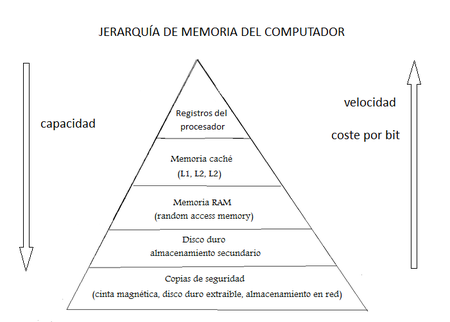
\includegraphics[scale=1]{images/jerarquia-de-memoria.png}
   \caption{Jerarquía de memoria}
   \label{speedup}
\end{figure}

En la jerarquía de memoria de un computador, los componentes más rápidos son también los que menos capacidad tienen y los más caros. Cuando un programa se ejecuta, dependiendo de la cantidad de almacenamiento que necesite, utilizan los distintos recursos de la jerarquía según cuánto necesite almacenar y según la disponibilidad de los mismos.

\vspace{4mm}
Rayo y Centella cuentan con las siguientes características:

\begin{center}
\begin{tabu} to 0.8\textwidth { | X[l] | X[l] | X[l] | X[l] | X[l] | }
 \hline
 \multicolumn{1}{|c|}{\bf Máquina} & \multicolumn{1}{|c|}{\bf L1} & \multicolumn{1}{|c|}{\bf L2} &  \multicolumn{1}{|c|}{\bf L3} &  \multicolumn{1}{|c|}{\bf RAM} \\
 \hline
 Rayo & \centering 1536KiB & \centering 6MiB & \centering 10MiB  & \centering 64GB\\
  \hline
   Centella &  \centering 576KiB & \centering 12MiB & \centering 12MiB & \centering 64GB \\
 \hline
\end{tabu}
\end{center}

En todas las gráficas generadas se obtienen una serie de resultados en común.

\begin{itemize}
 \item  En las gráficas de tiempo de ejecución, se puede observar que Centella realiza los cálculos más rápido que Rayo. Sin embargo, cuanto más aumenta el número de procesadores, ambas máquinas tienden a tener un tiempo de ejecución similar.
 \item  En las gráficas de la aceleración, la eficiencia, la utilización, la redundancia y la calidad del paralelismo, Rayo aparece generalmente por encima de Centella. Esto no significa que Rayo sea más potente ni más rápido, sino que Rayo se ve mucho más beneficiado de la ejecución paralela que Centella.
 \item Tanto para Rayo como para Centella ocurre speedup superlineal en la mayoría de algoritmos. Esto es así porque, tras utilizar un número determinado de procesadores, el tamaño del problema cabe en caché, que implica evitar el acceso a memoria RAM y, por tanto, acelerar muchísimo más los cálculos.
\end{itemize}

Los tamaños de problema para cada algoritmo son:

\begin{center}
\begin{tabular}{|l|l|l|l|l|}
\hline
Algoritmo & \multicolumn{4}{c|}{Tamaño de problema C} \\ \hline
IS        & \multicolumn{4}{l|}{$ 2^{27} $ claves con valor máximo de $ 2^{23} $}     \\ \hline
EP        & \multicolumn{4}{l|}{$ 2^{32} $ pares de números aleatorios}                   \\ \hline
CG        & \multicolumn{4}{l|}{150000 filas, 75 iteraciones, 15 no ceros}                   \\ \hline
MG        & \multicolumn{4}{l|}{Matriz 512 x 512 x 512, 20 iteraciones}                   \\ \hline
FT        & \multicolumn{4}{l|}{Matriz 512 x 512 x 512, 20 iteraciones}                   \\ \hline
BT        & \multicolumn{4}{l|}{Matriz 162 x 162 x 162, 200 iteraciones}                   \\ \hline
SP        & \multicolumn{4}{l|}{Matriz 162 x 162 x 162, 400 iteraciones}                   \\ \hline
LU        & \multicolumn{4}{l|}{Matriz 480 x 320 x 28, 0.8GB de memoria necesaria}                   \\ \hline
\end{tabular}
\end{center}

De todos los algoritmos, el que menos tiempo tardó en ejecutarse de media fue el de IS (Figura \ref{is:tiempo} y el que más el algoritmo de BT, matrices tridiagonales en bloque (Figura \ref{bt:tiempo}).

\vspace{2mm}

Una de las gráficas que llama más la atención es la de la Calidad del Paralelismo (Figura \ref{cg:calidad}), especialmente Centella. En este caso, Centella presenta un buen speed up (Figura \ref{cg:speedup}) y una buena eficiencia (Figura \ref{cg:eficiencia}). Sin embargo, la redundancia es muy alta (Figura \ref{cg:redundancia}, por lo que la calidad del paralelismo es mala.

\newpage

\subsection{Gráficas IS}

\begin{center}
 \centering
 \begin{minipage}[b]{.49\textwidth}
  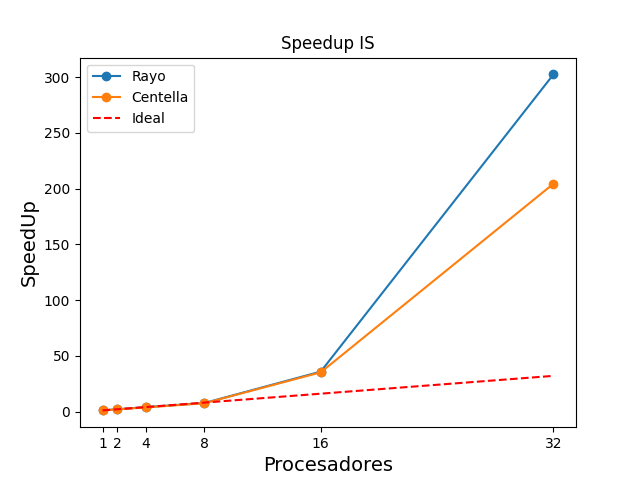
\includegraphics[width=1\linewidth]{plots/speed-up-is.png}
  \captionof{figure}{Speedup IS}
  \label{is:speedup}
 \end{minipage}
% \qquad
 \begin{minipage}[b]{.49\textwidth}
  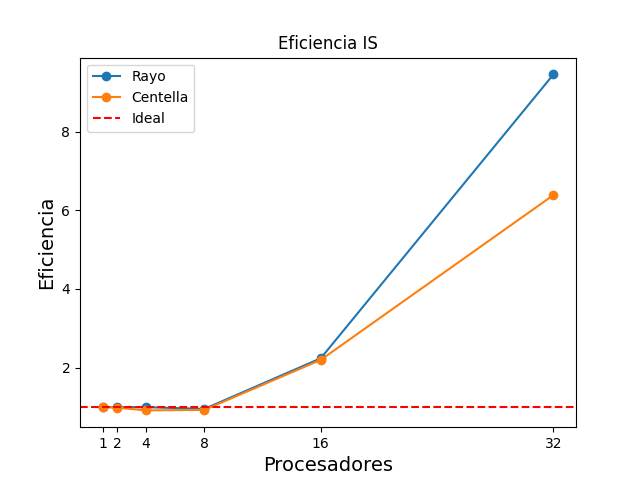
\includegraphics[width=1\linewidth]{plots/efficiency-is.png}
  \captionof{figure}{Eficiencia IS}
 \end{minipage}
\end{center}

\begin{center}
 \centering
  \begin{minipage}[b]{.49\textwidth}
  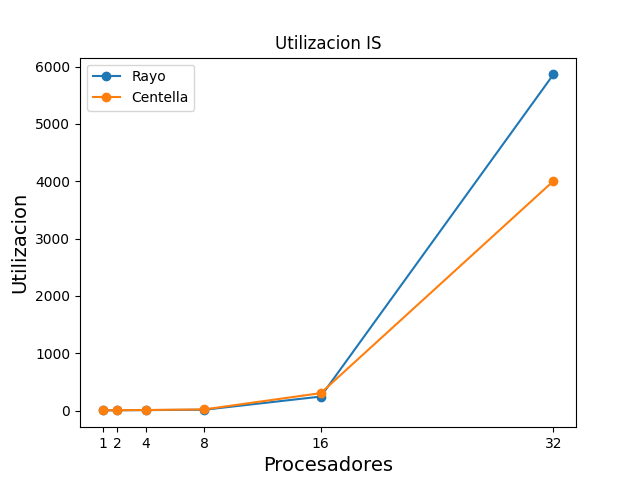
\includegraphics[width=1\linewidth]{plots/utilizacion-is.png}
  \captionof{figure}{Utilización IS}
 \end{minipage}
% \qquad
 \begin{minipage}[b]{.49\textwidth}
  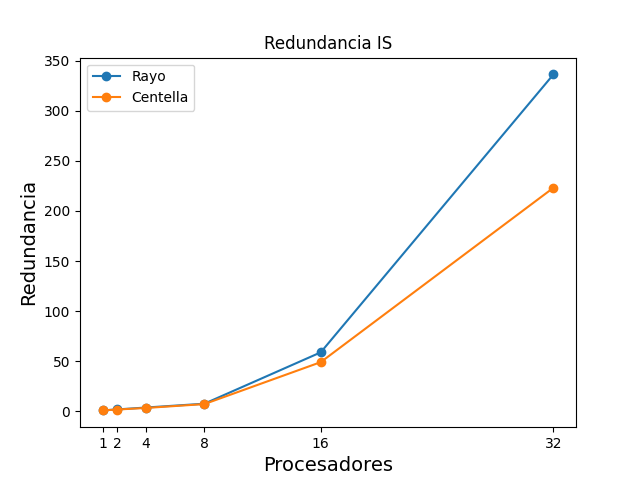
\includegraphics[width=1\linewidth]{plots/redundancy-is.png}
  \captionof{figure}{Redundancia IS}
 \end{minipage}
\end{center}

\begin{center}
 \centering
 \begin{minipage}[b]{.49\textwidth}
  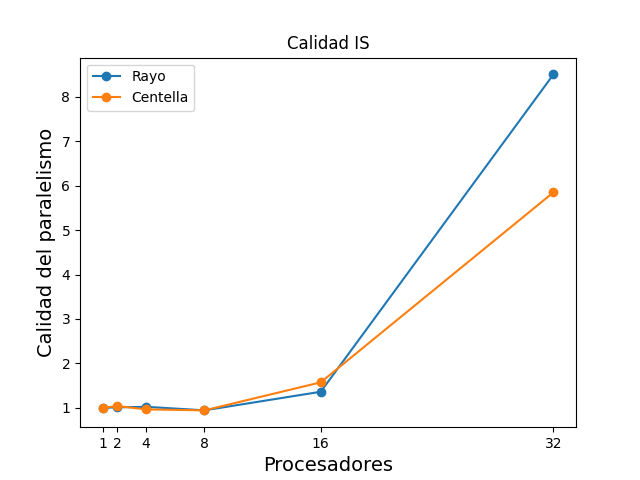
\includegraphics[width=1\linewidth]{plots/calidad-is.png}
  \captionof{figure}{Calidad Paralelismo IS}
 \end{minipage}
   % \qquad
 \begin{minipage}[b]{.49\textwidth}
  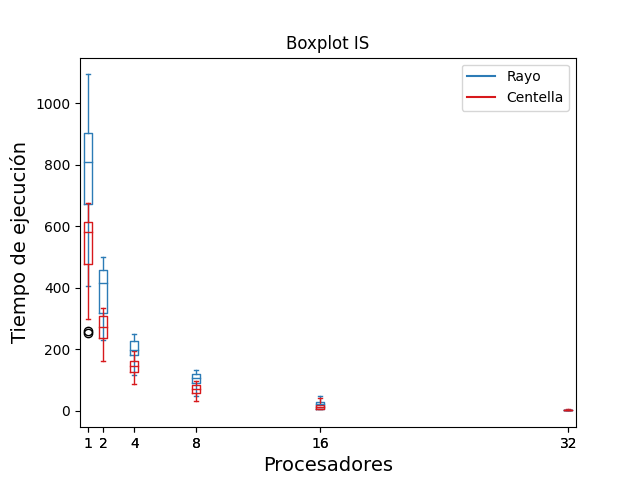
\includegraphics[width=1\linewidth]{plots/boxplot-is.png}
  \captionof{figure}{Tiempo Ejecución IS}
  \label{is:tiempo}
 \end{minipage}
\end{center}

\newpage

\subsection{Gráficas EP}

\begin{center}
 \centering
 \begin{minipage}[b]{.49\textwidth}
  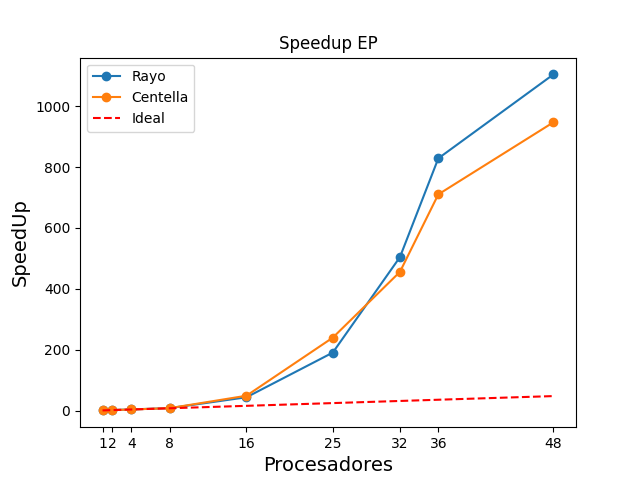
\includegraphics[width=1\linewidth]{plots/speed-up-ep.png}
  \captionof{figure}{Speedup EP}
  \label{ep:speedup}
 \end{minipage}
% \qquad
 \begin{minipage}[b]{.49\textwidth}
  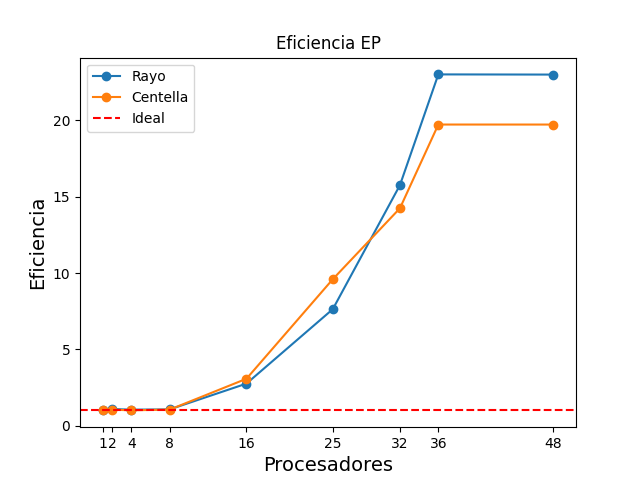
\includegraphics[width=1\linewidth]{plots/efficiency-ep.png}
  \captionof{figure}{Eficiencia EP}
 \end{minipage}
\end{center}

\begin{center}
 \centering
  \begin{minipage}[b]{.49\textwidth}
  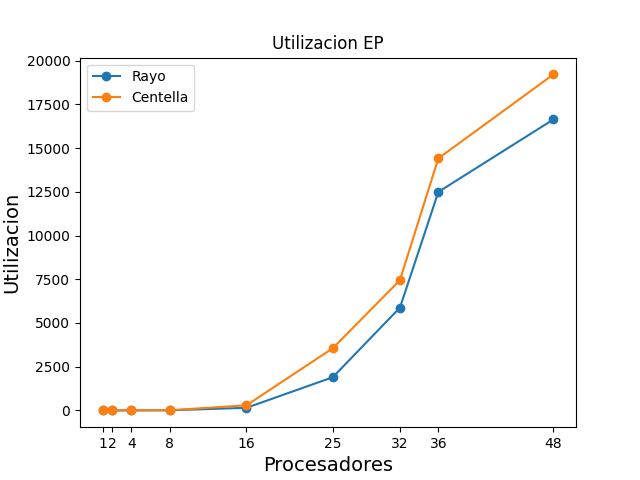
\includegraphics[width=1\linewidth]{plots/utilizacion-ep.png}
  \captionof{figure}{Utilización EP}
 \end{minipage}
% \qquad
 \begin{minipage}[b]{.49\textwidth}
  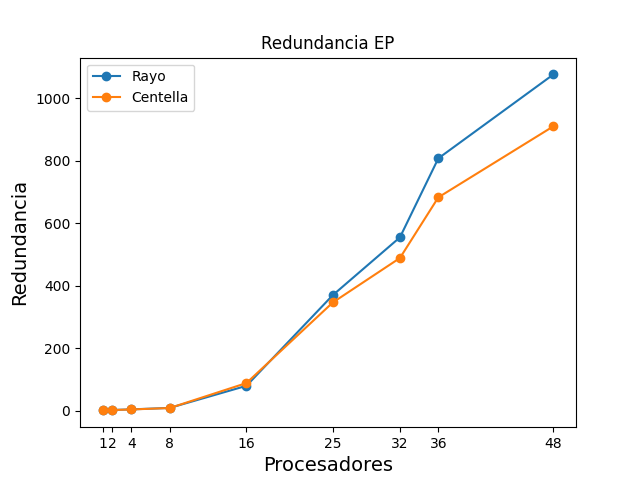
\includegraphics[width=1\linewidth]{plots/redundancy-ep.png}
  \captionof{figure}{Redundancia EP}
 \end{minipage}
\end{center}

\begin{center}
 \centering
 \begin{minipage}[b]{.49\textwidth}
  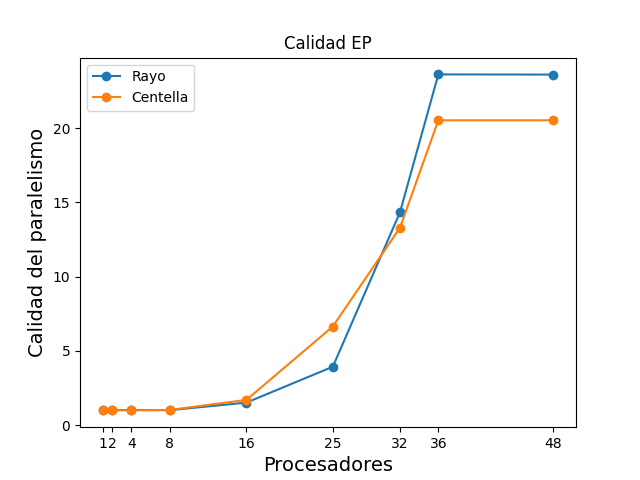
\includegraphics[width=1\linewidth]{plots/calidad-ep.png}
  \captionof{figure}{Calidad Paralelismo EP}
 \end{minipage}
  % \qquad
 \begin{minipage}[b]{.49\textwidth}
  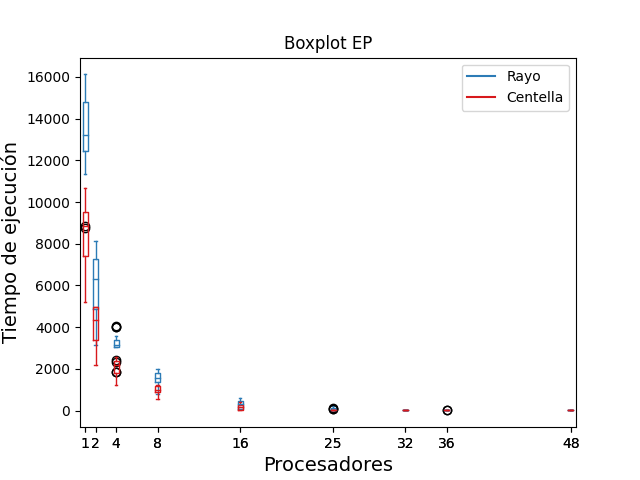
\includegraphics[width=1\linewidth]{plots/boxplot-ep.png}
  \captionof{figure}{Tiempo Ejecución EP}
 \end{minipage}
\end{center}

\newpage

\subsection{Gráficas CG}

\begin{center}
 \centering
 \begin{minipage}[b]{.49\textwidth}
  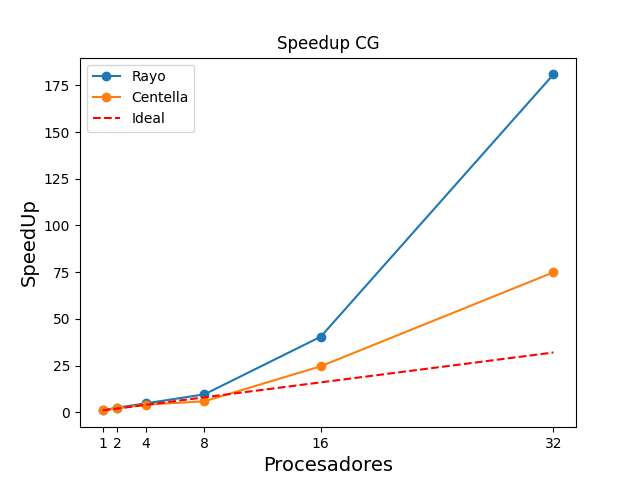
\includegraphics[width=1\linewidth]{plots/speed-up-cg.png}
  \label{cg:speedup}
  \captionof{figure}{Speedup CG}
 \end{minipage}
% \qquad
 \begin{minipage}[b]{.49\textwidth}
  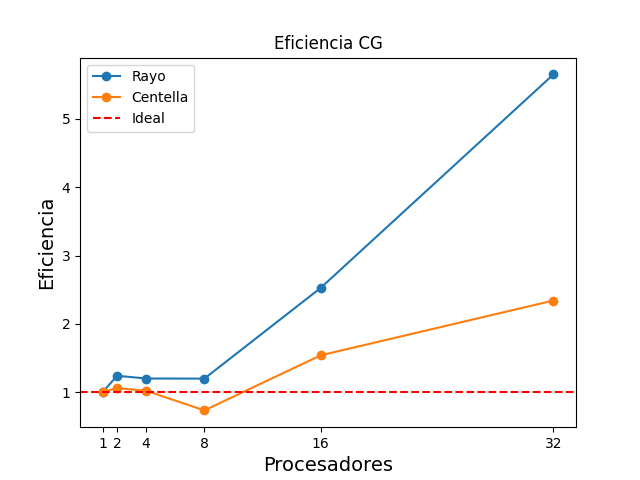
\includegraphics[width=1\linewidth]{plots/efficiency-cg.png}
  \captionof{figure}{Eficiencia CG}
    \label{cg:eficiencia}
 \end{minipage}
\end{center}

\begin{center}
 \centering
  \begin{minipage}[b]{.49\textwidth}
  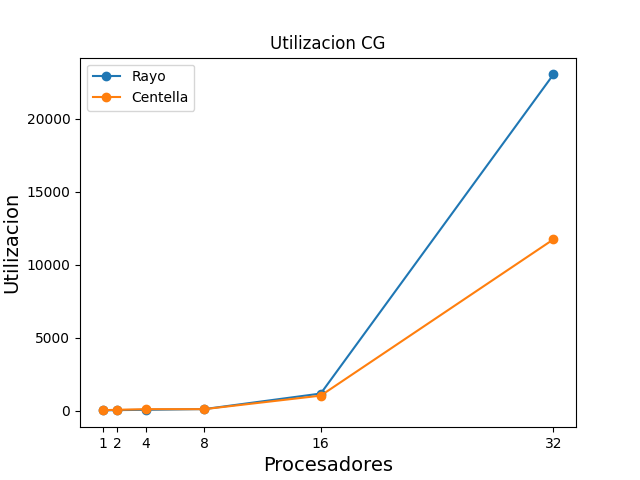
\includegraphics[width=1\linewidth]{plots/utilizacion-cg.png}
  \captionof{figure}{Utilización CG}
 \end{minipage}
% \qquad
 \begin{minipage}[b]{.49\textwidth}
  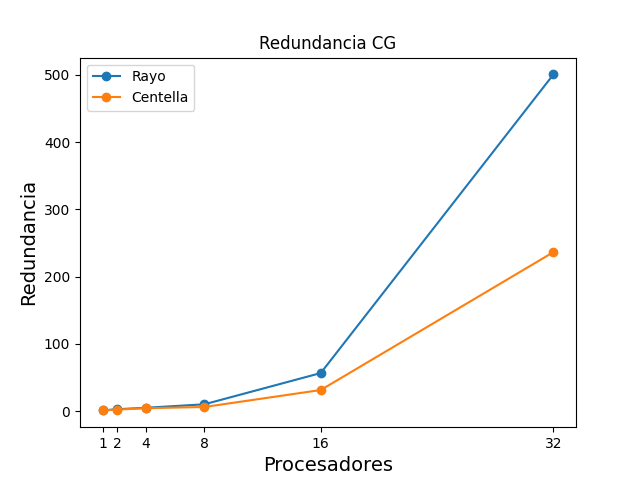
\includegraphics[width=1\linewidth]{plots/redundancy-cg.png}
  \captionof{figure}{Redundancia CG}
    \label{cg:redundancia}
 \end{minipage}
\end{center}

\begin{center}
 \centering
 \begin{minipage}[b]{.49\textwidth}
  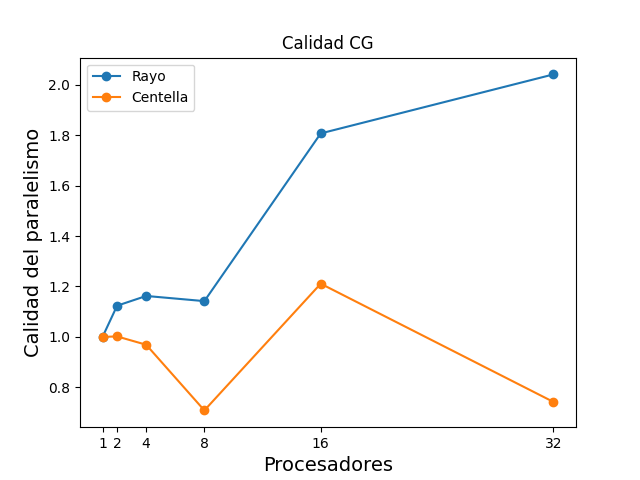
\includegraphics[width=1\linewidth]{plots/calidad-cg.png}
  \captionof{figure}{Calidad Paralelismo CG}
    \label{cg:calidad}
 \end{minipage}
  % \qquad
 \begin{minipage}[b]{.49\textwidth}
  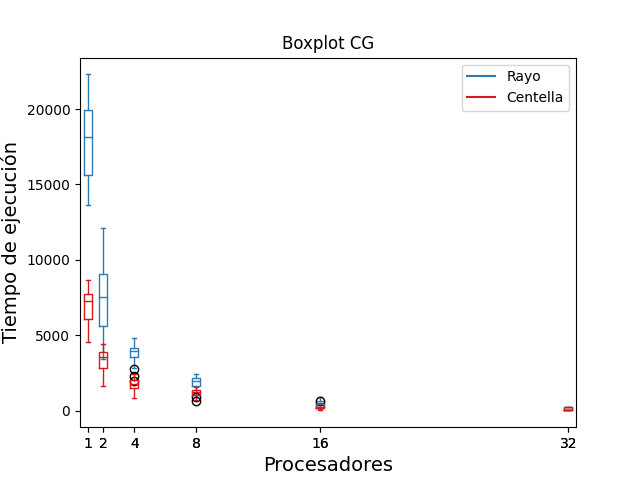
\includegraphics[width=1\linewidth]{plots/boxplot-cg.png}
    \label{cg:tiempo}
  \captionof{figure}{Tiempo Ejecución CG}
 \end{minipage}
\end{center}

\newpage

\subsection{Gráficas MG}

\begin{center}
 \centering
 \begin{minipage}[b]{.49\textwidth}
  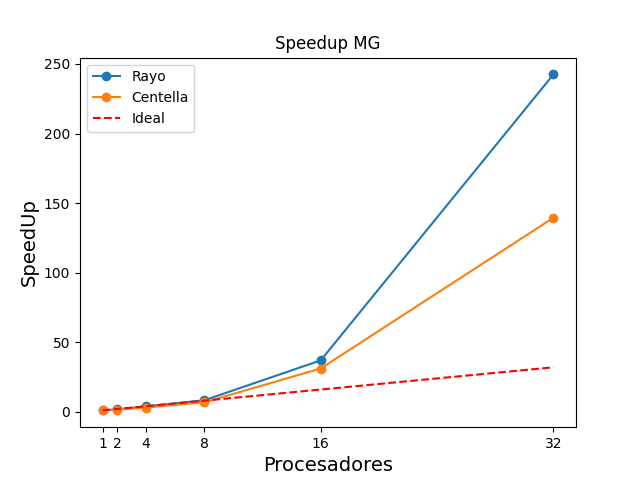
\includegraphics[width=1\linewidth]{plots/speed-up-mg.png}
  \captionof{figure}{Speedup MG}
 \end{minipage}
% \qquad
 \begin{minipage}[b]{.49\textwidth}
  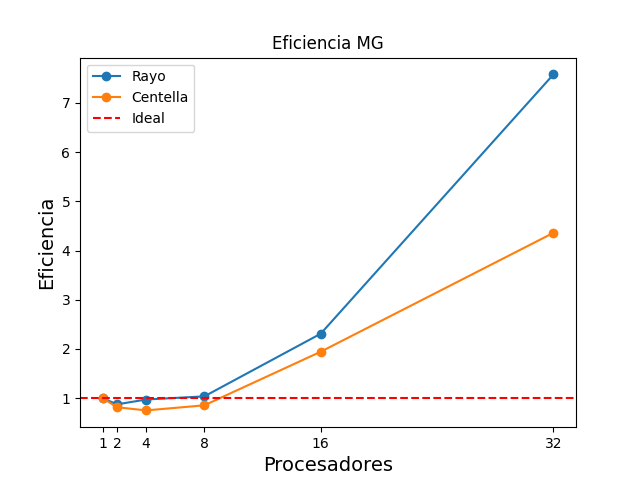
\includegraphics[width=1\linewidth]{plots/efficiency-mg.png}
  \captionof{figure}{Eficiencia MG}
 \end{minipage}
\end{center}

\begin{center}
 \centering
  \begin{minipage}[b]{.49\textwidth}
  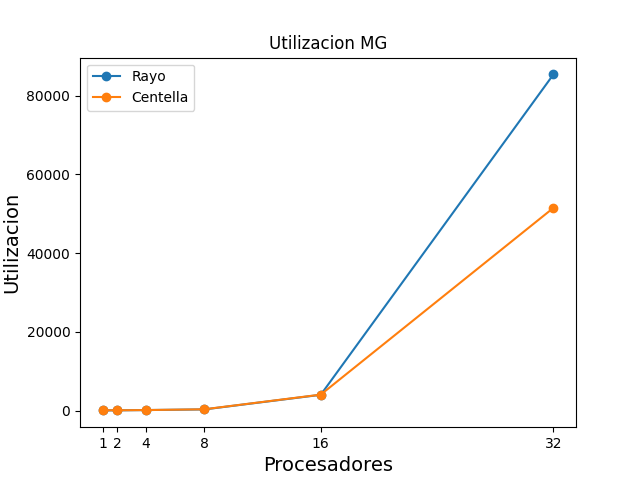
\includegraphics[width=1\linewidth]{plots/utilizacion-mg.png}
  \captionof{figure}{Utilización MG}
 \end{minipage}
% \qquad
 \begin{minipage}[b]{.49\textwidth}
  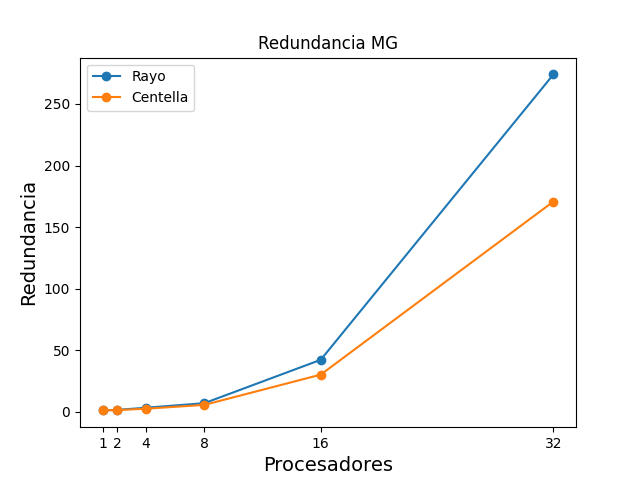
\includegraphics[width=1\linewidth]{plots/redundancy-mg.png}
  \captionof{figure}{Redundancia MG}
 \end{minipage}
\end{center}

\begin{center}
 \centering
 \begin{minipage}[b]{.49\textwidth}
  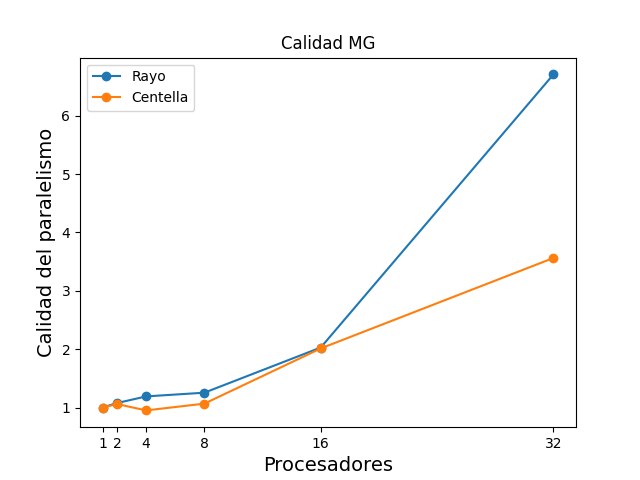
\includegraphics[width=1\linewidth]{plots/calidad-mg.png}
  \captionof{figure}{Calidad Paralelismo MG}
 \end{minipage}
  % \qquad
 \begin{minipage}[b]{.49\textwidth}
  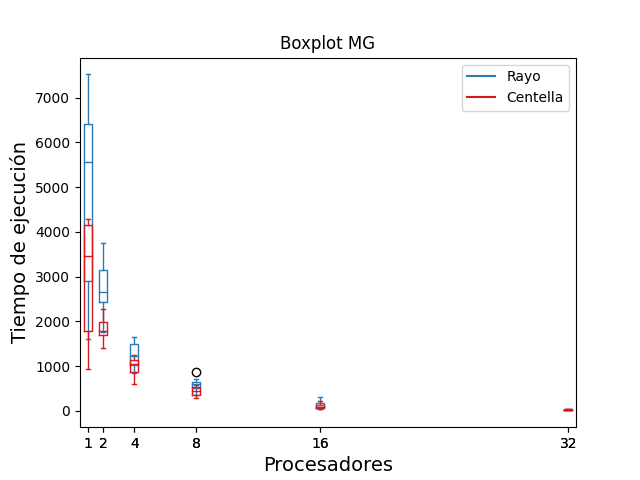
\includegraphics[width=1\linewidth]{plots/boxplot-mg.png}
  \captionof{figure}{Tiempo Ejecución MG}
 \end{minipage}
\end{center}

\newpage

\subsection{Gráficas FT}

\begin{center}
 \centering
 \begin{minipage}[b]{.49\textwidth}
  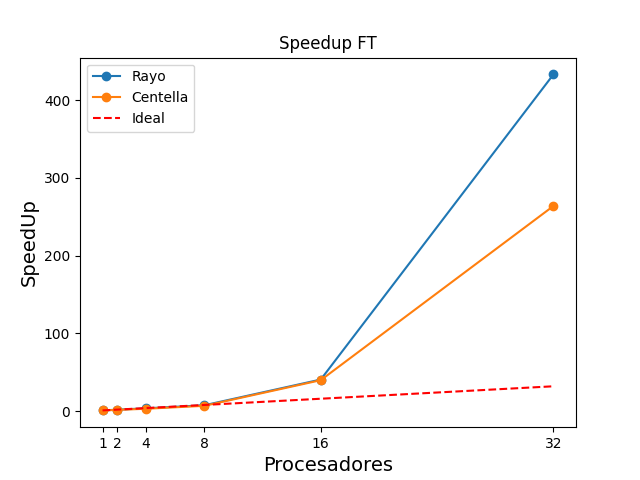
\includegraphics[width=1\linewidth]{plots/speed-up-ft.png}
  \captionof{figure}{Speedup FT}
  \label{ft:speedup}
 \end{minipage}
% \qquad
 \begin{minipage}[b]{.49\textwidth}
  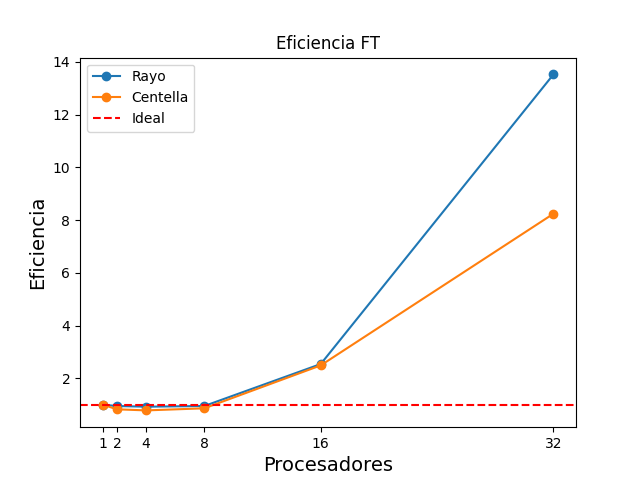
\includegraphics[width=1\linewidth]{plots/efficiency-ft.png}
  \captionof{figure}{Eficiencia FT}
 \end{minipage}
\end{center}

\begin{center}
 \centering
  \begin{minipage}[b]{.49\textwidth}
  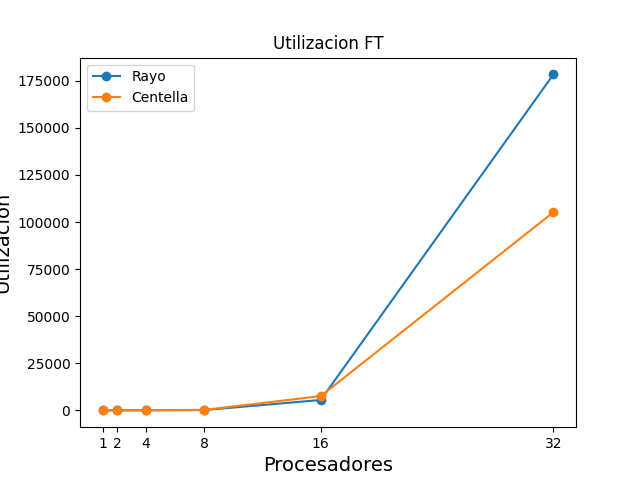
\includegraphics[width=1\linewidth]{plots/utilizacion-ft.png}
  \captionof{figure}{Utilización FT}
 \end{minipage}
% \qquad
 \begin{minipage}[b]{.49\textwidth}
  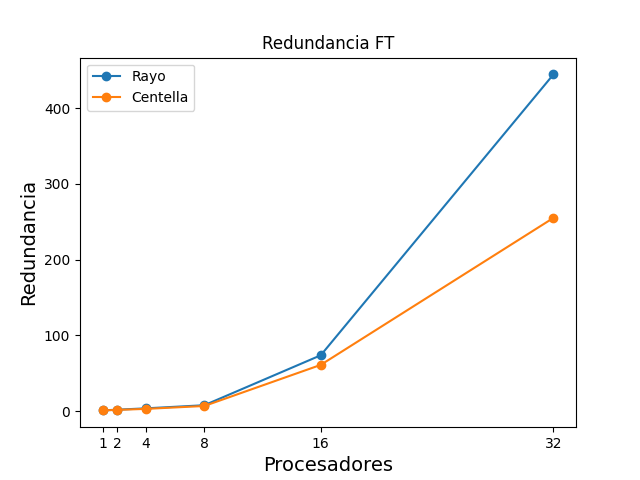
\includegraphics[width=1\linewidth]{plots/redundancy-ft.png}
  \captionof{figure}{Redundancia FT}
 \end{minipage}
\end{center}

\begin{center}
 \centering
 \begin{minipage}[b]{.49\textwidth}
  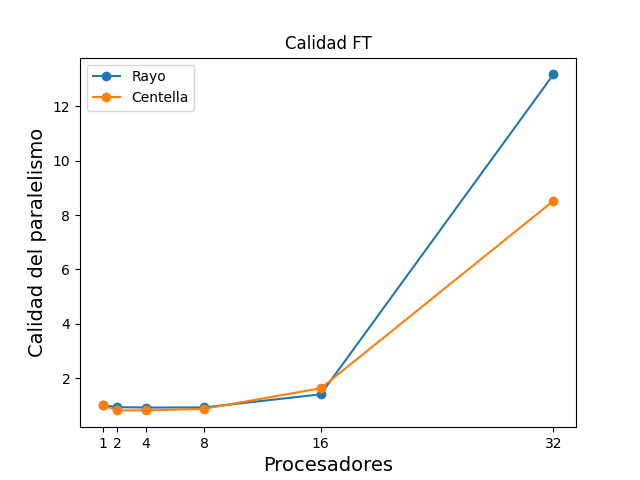
\includegraphics[width=1\linewidth]{plots/calidad-ft.png}
  \captionof{figure}{Calidad Paralelismo FT}
 \end{minipage}
  % \qquad
 \begin{minipage}[b]{.49\textwidth}
  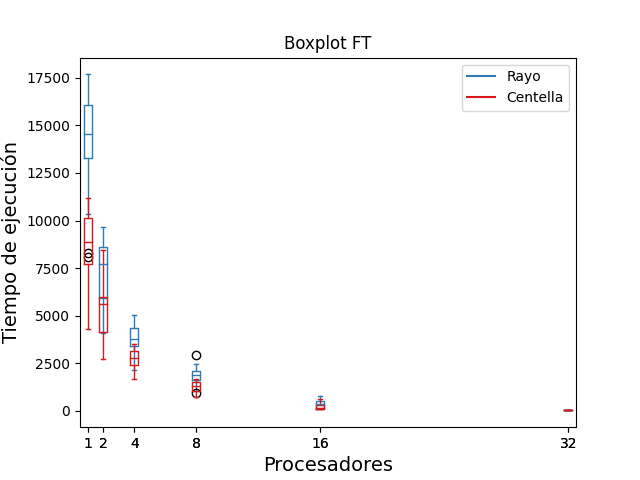
\includegraphics[width=1\linewidth]{plots/boxplot-ft.png}
  \captionof{figure}{Tiempo Ejecución FT}
 \end{minipage}
\end{center}

\newpage

\subsection{Gráficas BT}

\begin{center}
 \centering
 \begin{minipage}[b]{.49\textwidth}
  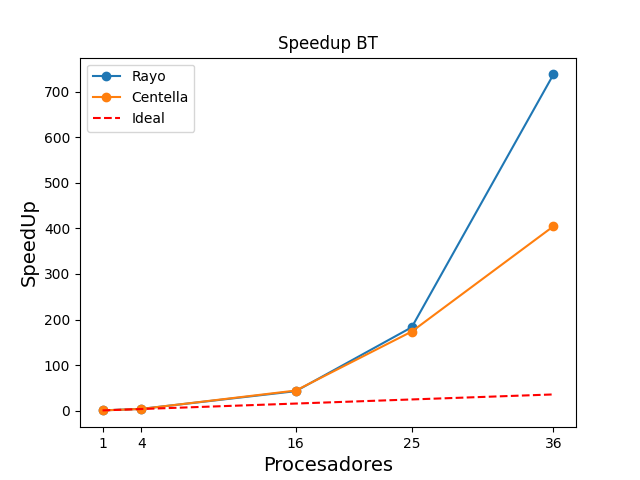
\includegraphics[width=1\linewidth]{plots/speed-up-bt.png}
  \captionof{figure}{Speedup BT}
 \end{minipage}
% \qquad
 \begin{minipage}[b]{.49\textwidth}
  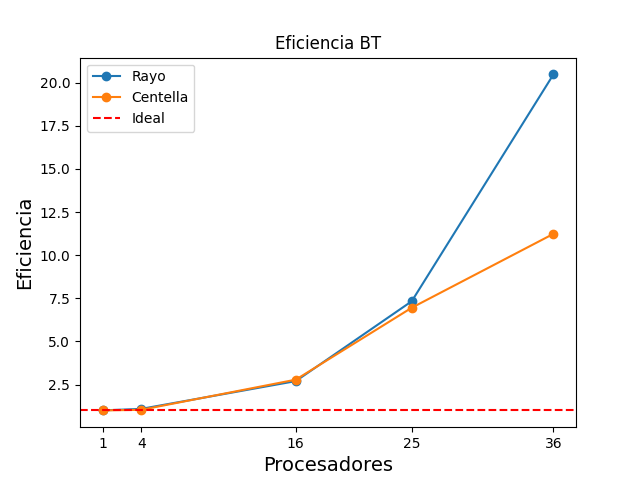
\includegraphics[width=1\linewidth]{plots/efficiency-bt.png}
  \captionof{figure}{Eficiencia BT}
 \end{minipage}
\end{center}

\begin{center}
 \centering
  \begin{minipage}[b]{.49\textwidth}
  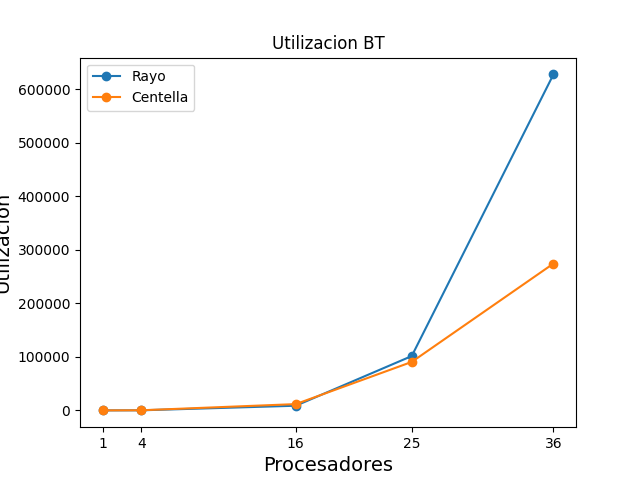
\includegraphics[width=1\linewidth]{plots/utilizacion-bt.png}
  \captionof{figure}{Utilización BT}
 \end{minipage}
% \qquad
 \begin{minipage}[b]{.49\textwidth}
  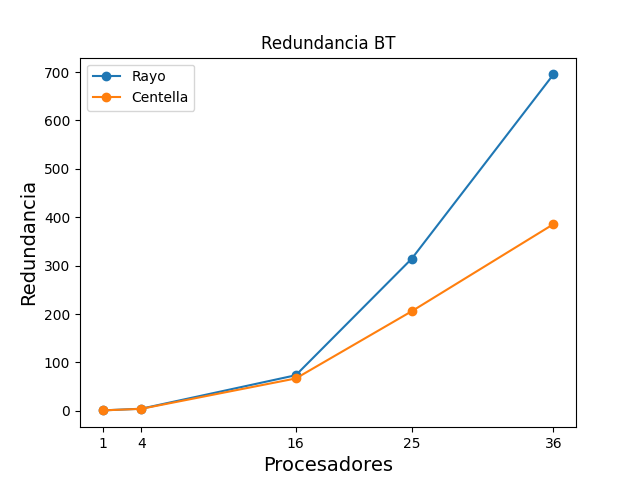
\includegraphics[width=1\linewidth]{plots/redundancy-bt.png}
  \captionof{figure}{Redundancia BT}
 \end{minipage}
\end{center}

\begin{center}
 \centering
 \begin{minipage}[b]{.49\textwidth}
  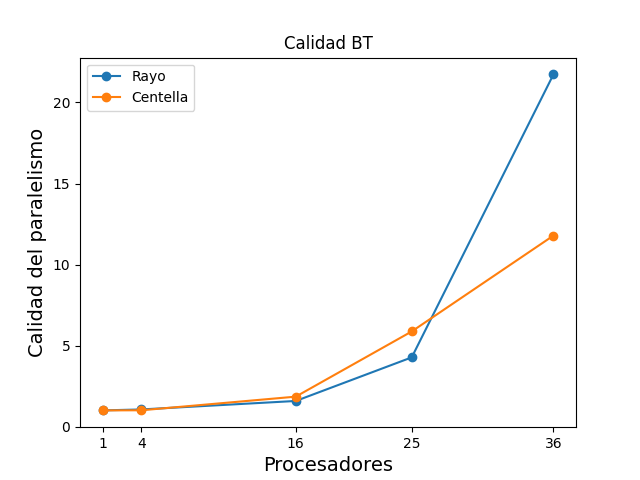
\includegraphics[width=1\linewidth]{plots/calidad-bt.png}
  \captionof{figure}{Calidad Paralelismo BT}
 \end{minipage}
  % \qquad
 \begin{minipage}[b]{.49\textwidth}
  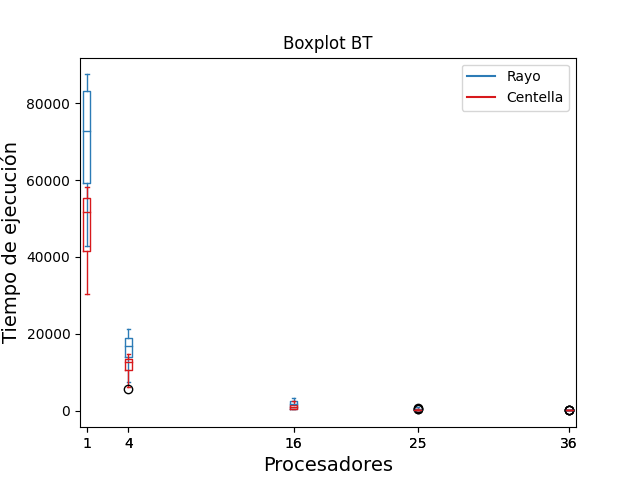
\includegraphics[width=1\linewidth]{plots/boxplot-bt.png}
  \label{bt:tiempo}
  \captionof{figure}{Tiempo Ejecución BT}
 \end{minipage}
\end{center}

\newpage

\subsection{Gráficas SP}

\begin{center}
 \centering
 \begin{minipage}[b]{.49\textwidth}
  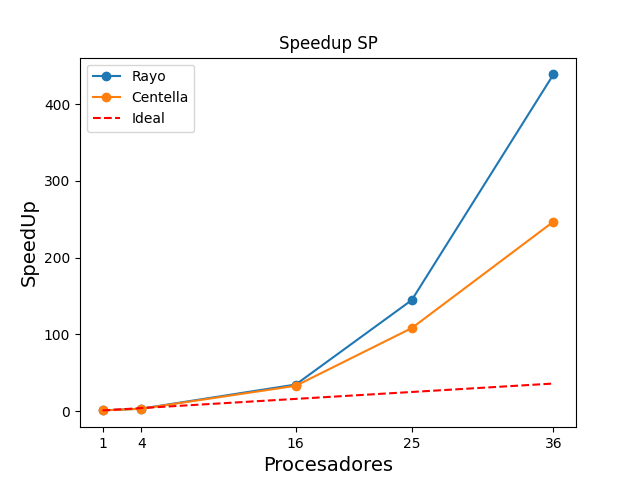
\includegraphics[width=1\linewidth]{plots/speed-up-sp.png}
  \captionof{figure}{Speedup SP}
 \end{minipage}
% \qquad
 \begin{minipage}[b]{.49\textwidth}
  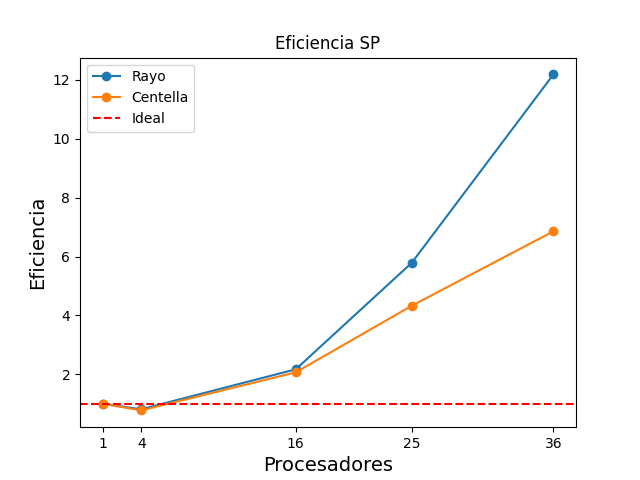
\includegraphics[width=1\linewidth]{plots/efficiency-sp.png}
  \captionof{figure}{Eficiencia SP}
 \end{minipage}
\end{center}

\begin{center}
 \centering
  \begin{minipage}[b]{.49\textwidth}
  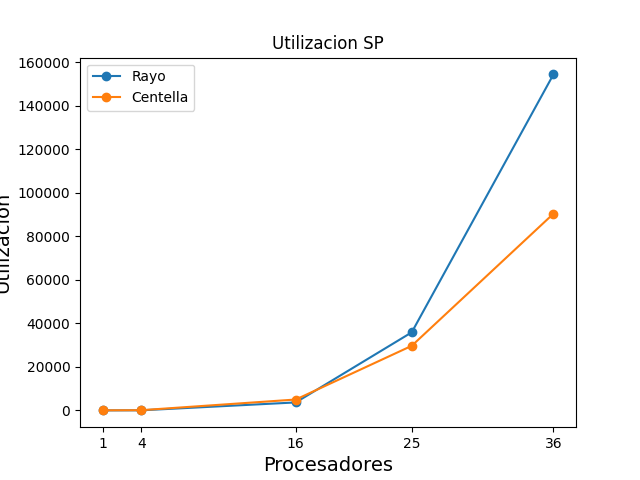
\includegraphics[width=1\linewidth]{plots/utilizacion-sp.png}
  \captionof{figure}{Utilización SP}
 \end{minipage}
% \qquad
 \begin{minipage}[b]{.49\textwidth}
  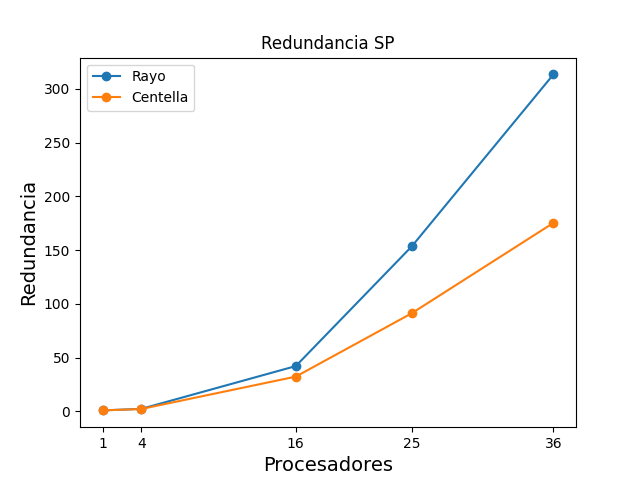
\includegraphics[width=1\linewidth]{plots/redundancy-sp.png}
  \captionof{figure}{Redundancia SP}
 \end{minipage}
\end{center}

\begin{center}
 \centering
 \begin{minipage}[b]{.49\textwidth}
  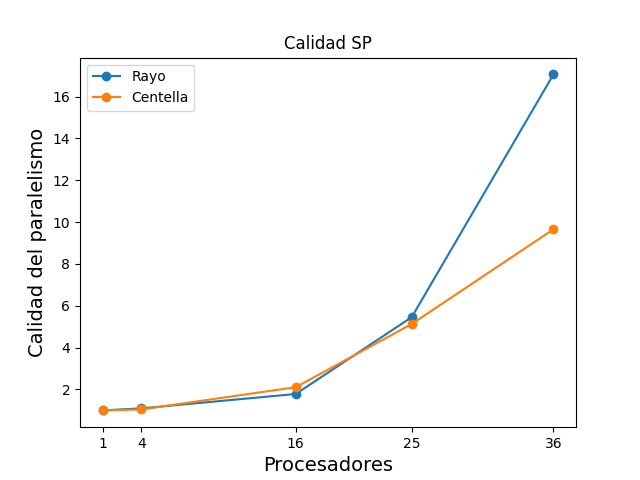
\includegraphics[width=1\linewidth]{plots/calidad-sp.png}
  \captionof{figure}{Calidad Paralelismo SP}
 \end{minipage}
  % \qquad
 \begin{minipage}[b]{.49\textwidth}
  \includegraphics[width=1\linewidth]{plots/boxplot-sp.png}
  \captionof{figure}{Tiempo Ejecución SP}
 \end{minipage}
\end{center}

\newpage

\subsection{Gráficas LU}

\begin{center}
 \centering
 \begin{minipage}[b]{.49\textwidth}
  \includegraphics[width=1\linewidth]{plots/speed-up-lu.png}
  \captionof{figure}{Speedup LU}
 \end{minipage}
% \qquad
 \begin{minipage}[b]{.49\textwidth}
  \includegraphics[width=1\linewidth]{plots/efficiency-lu.png}
  \captionof{figure}{Eficiencia LU}
 \end{minipage}
\end{center}

\begin{center}
 \centering
  \begin{minipage}[b]{.49\textwidth}
  \includegraphics[width=1\linewidth]{plots/utilizacion-lu.png}
  \captionof{figure}{Utilización LU}
 \end{minipage}
% \qquad
 \begin{minipage}[b]{.49\textwidth}
  \includegraphics[width=1\linewidth]{plots/redundancy-lu.png}
  \captionof{figure}{Redundancia LU}
 \end{minipage}
\end{center}

\begin{center}
 \centering
 \begin{minipage}[b]{.49\textwidth}
  \includegraphics[width=1\linewidth]{plots/calidad-LU.png}
  \captionof{figure}{Calidad Paralelismo LU}
 \end{minipage}
 % \qquad
 \begin{minipage}[b]{.49\textwidth}
  \includegraphics[width=1\linewidth]{plots/boxplot-lu.png}
  \captionof{figure}{Tiempo Ejecución LU}
 \end{minipage}
\end{center}


%%%%%%%%%%%%%%%%%%%%%%%%%%%%%%%%%%%%%%%%%%%%%%%%%%%%%%%%%
\newpage{\pagestyle{empty}}
\thispagestyle{empty}

\chapter{\LARGE Conclusiones y líneas futuras}
\label{chapter:Resultados}

\section{Conclusiones}

La computación de altas prestaciones está a la última orden del día. La tendencia del mundo actual es seguir mejorando y exprimiendo al máximo el potencial de la tecnología, con el fin de avanzar en la ciencia.
\vspace{2mm}

Dos tendencias actuales lo confirman: el desarrollo de ordenadores cuánticos e instalación de más supercomputadores por el mundo y, quizás la más desapercibida, los desarrollos de vacunas del coronavirus, descubrimientos y estudios continuos en astronomía y el modelado del tiempo para su predicción. 
\vspace{2mm}

Implementar un sistema de computación de altas prestaciones es relativamente sencillo. Aunque existen diversas soluciones empresariales, es posible crearse un sistema propio combinando distintas herramientas gratuitas y de código libre, a cambio del tiempo que cuesta implementar y depurar y el precio a pagar por las máquinas y su mantenimiento energético mensual.
\vspace{2mm}

Como mantener múltiples sistemas puede ser una labor tediosa, es conveniente seguir una serie de buenas prácticas. Esencialmente, se puede resumir en que las tareas relacionadas con sistemas solo se tengan que hacer una única vez, independientemente cuánto de grande sea el sistema. Por eso, es conveniente tener todos los recursos centralizados y compartidos con los distintos nodos, así como disponer en cada nodo únicamente lo necesario para ejercer su función dentro del \emph{cluster}.

\section{Líneas futuras}

El trabajo se puede continuar por diversas líneas.
\vspace{4mm}

En primer lugar, se puede ampliar el sistema con más nodos de cómputo que, incluso, podrían incluir alguna tarjeta gráfica para calcular modelos de inteligencia artificial o realizar grandes operaciones con un gran volumen de datos, así como ampliar el software proporcionado en el \emph{cluster}.
\vspace{4mm}

Por otro lado, se puede utilizar Ansible \cite{ansible} y preparar con él algún script para actualizar todos los sistemas a su última versión y automatizar la configuración de un nuevo nodo.
\vspace{4mm}

Por último, se podría incorporar Slurm Web \cite{slurmweb}, para visualizar de manera gráfica el estado y la disponibilidad de los recursos, los trabajos que se encuentran en cola y aquellos que están ejecutándose.


%%%%%%%%%%%%%%%%%%%%%%%%%%%%%%%%%%%%%%%%%%%%%%%%%%%%%%%%%
\newpage{\pagestyle{empty}}
\thispagestyle{empty}

\chapter{\LARGE Summary and Conclusions}
\label{chapter:Conclusiones}

This chapter is compulsory. The memory should include an extended summary and conclusions in english. 

%%%%%%%%%%%%%%%%%%%%%%%%%%%%%%%%%%%%%%%%%%%%%%%%%%%%%%%%%
\newpage{\pagestyle{empty}}
\thispagestyle{empty}

\chapter{\LARGE Presupuesto}
\label{chapter:presupuesto}

En este capítulo se realiza un presupuesto del trabajo realizado. Todas las herramientas utilizadas son gratuitas, por lo que el presupuesto necesario para este proyecto está definido por el material necesario y el sueldo del administrador de sistemas durante 4 meses (tiempo de duración de la asignatura).
\vspace{2mm}

Para el presupuesto de los servidores, se tomó de referencia una factura de la compra realizada por el departamento en 2014. Cabe a destacar que el precio del mismo modelo de servidor en el año de la realización de este trabajo (2021) es considerablemente más barato.

\section{Presupuesto}

\begin{center}
\begin{tabu} to 0.8\textwidth { | X[l] | X[l] | X[l] | }
 \hline
 \multicolumn{1}{|c|}{\bf Material} & \multicolumn{1}{|c|}{\bf Cantidad} & \multicolumn{1}{|c|}{\bf Presupuesto} \\
 \hline
 Servidor Dell PowerEdge R815 & \centering 3 & \centering 7.021€\\
  \hline
 Portatil de trabajo  & \centering 1 & \centering 800€\\
 \hline
   Total: &  & \centering 21.863€\\
 \hline
\end{tabu}
\end{center}

\begin{table}[htb]
   \centering
   \caption{Presupuesto del material}
   \label{chapter:presupuesto}
\end{table}

\begin{center}
\begin{tabu} to 0.8\textwidth { | X[l] | X[l] | X[l] | }
 \hline
 \multicolumn{1}{|c|}{\bf Personal} & \multicolumn{1}{|c|}{\bf Meses} & \multicolumn{1}{|c|}{\bf Presupuesto} \\
 \hline
 Ing. Informático & \centering 4 & \centering 1.200€ \\
  \hline
   Total: &  & \centering 4.800€\\
 \hline
\end{tabu}
\end{center}

\begin{table}[htb]
   \centering
   \caption{Presupuesto del personal}
   \label{chapter:presupuesto}
\end{table}

Para realizar este proyecto hicieron falta 4 meses y un precio final de 26.663€.

%%%%%%%%%%%%%%%%%%%%%%%%%%%%%%%%%%%%%%%%%%%%%%%%%%%%%%%%%
\newpage{\pagestyle{empty}\cleardoublepage}
\thispagestyle{empty}

\begin{appendix}

\chapter{\LARGE Título del Apéndice 1}
\label{appendix:1}
\section{Script administración de usuarios}
\label{Apendice1:XXX}

\begin{center}
\begin{footnotesize}
\begin{verbatim}
#!/bin/sh

show_help()
{
   # Display Help
   echo "Bash utility for cluster user management"
   echo
   echo "Syntax: cluster-user-management [a|m|d|u:]"
   echo "options:"
   echo " -h     		Print this Help."
   echo " -a <user>    		Create given user."
   echo " -m <user>    		Modify given user."
   echo " -d <user>    		Delete given user."
   echo " -q <quota>            Set user quota space. [20G default]"
   echo
   echo "Examples: "
   echo " - New user: -a test -q 25G"
   echo " - Modify user: -m test -q 500M"
   echo " - Delete user: -d test"
}

# $1 : username
# $2 : quota size (20G default)
add_user()
{
    if id -u "${1}" >/dev/null 2>&1; then
	    echo "[!] Ya existe el usuario ${1}."
	    return
    fi
	
    nscd --invalidate=passwd
    cpu useradd $1 -m  -p"${1}bolido"
    setquota -u $1 $2 $2 0 0 /home
    mkdir "/home/${1}/.ssh"
    ssh-keygen -t rsa -f "/home/${1}/.ssh/id_rsa" -q -N ""
    cp "/home/${1}/.ssh/id_rsa.pub" "/home/${1}/.ssh/authorized_keys"
    chown -R $1 "/home/${1}/.ssh" && chgrp -R $1 "/home/${1}/.ssh"
    echo "The password for user ${1} is: ${1}bolido"
}

# $1 : username
delete_user()
{
    cpu userdel -r $1
    cpu groupdel $1
    nscd --invalidate=passwd
}

# $1 : username
# $2 : quota size (20G default)
modify_user()
{
    setquota -u $1 $2 $2 0 0 /home
}

# A POSIX variable
OPTIND=1         # Reset in case getopts has been used previously in the shell.
OPERATION=
QUOTA="20G"
USERNAME=

if [ $# -eq 0 ]; then
    show_help
    exit 0
fi

while getopts "h?a:d:m:q:" opt; do
  case "$opt" in
    h|\?)
      show_help
      exit 0
      ;;
    a)  [ -n "$OPERATION" ] && show_help && exit || OPERATION="ADD_USER" && USERNAME=$OPTARG
      ;;
    d)  [ -n "$OPERATION" ] && show_help && exit || OPERATION="DELETE_USER" && USERNAME=$OPTARG
      ;;
    m)  [ -n "$OPERATION" ] && show_help && exit || OPERATION="MODIFY_USER" && USERNAME=$OPTARG
      ;;
    q) QUOTA=$OPTARG
      ;;
  esac
done

shift $((OPTIND-1))

[ "${1:-}" = "--" ] && shift

[ -z "$USERNAME" ] && show_help && exit

case $OPERATION in
    ADD_USER) add_user $USERNAME $QUOTA;;
    DELETE_USER) delete_user $USERNAME;;
    MODIFY_USER) modify_user $USERNAME $QUOTA;;
esac
\end{verbatim}
\end{footnotesize}
\end{center}\vspace{4mm}


\chapter{\LARGE Título del Apéndice 2}
\label{appendix:2}
\section{Script generador CSV}
\label{Apendice2:XXX}

\begin{center}
\begin{footnotesize}
\begin{verbatim}
#!/bin/bash

LOGS_DIR="/home/pladmin/pruebas/scripts/output/"
PARSED_LOGS_OUTPUT="/home/pladmin/pruebas/parsed-output/"
LOGS_FILES=$(ls $LOGS_DIR)
FILE_DELIMITER="EJECUCION DE"
file=$(echo "$LOGS_FILES" | head -n 1)
FILE_NAMES=($(cat $LOGS_DIR/$file | grep "$FILE_DELIMITER" | cut -d " " -f 3))

for file in $LOGS_FILES;
do
	delimiters=($(cat ${LOGS_DIR}${file} | grep -n "EJECUCION DE" | cut -d ":" -f 1))
	node=$(echo $file | cut -d "-" -f 1)
	echo "EJECUCION DE ${file}" >> ${PARSED_LOGS_OUTPUT}$node-${FILE_NAMES[0]}
 	sed -n "$(( ${delimiters[0]}+1 )), $(( ${delimiters[1]}-1 ))p" "${LOGS_DIR}${file}" >> ${PARSED_LOGS_OUTPUT}$node-${FILE_NAMES[0]}
        echo '$(( ${delimiters[0]}+1 )), $(( ${delimiters[1]}-1 ))p' "${LOGS_DIR}${file}"
	echo "EJECUCION DE ${file}" >> ${PARSED_LOGS_OUTPUT}$node-${FILE_NAMES[1]}
	sed -n "$(( ${delimiters[1]}+1 )), $(( ${delimiters[2]}-1 ))p" "${LOGS_DIR}${file}" >> ${PARSED_LOGS_OUTPUT}$node-${FILE_NAMES[1]}
        echo "EJECUCION DE ${file}" >> ${PARSED_LOGS_OUTPUT}$node-${FILE_NAMES[2]}
	sed -n "$(( ${delimiters[2]}+1 )), $(( ${delimiters[3]}-1 ))p" "${LOGS_DIR}${file}" >> ${PARSED_LOGS_OUTPUT}$node-${FILE_NAMES[2]}
        echo "EJECUCION DE ${file}" >> ${PARSED_LOGS_OUTPUT}$node-${FILE_NAMES[3]}
	sed -n "$(( ${delimiters[3]}+1 )), $(( ${delimiters[4]}-1 ))p" "${LOGS_DIR}${file}" >> ${PARSED_LOGS_OUTPUT}$node-${FILE_NAMES[3]}
        echo "EJECUCION DE ${file}" >> ${PARSED_LOGS_OUTPUT}$node-${FILE_NAMES[4]}
	sed -n "$(( ${delimiters[4]}+1 )), $(( ${delimiters[5]}-1 ))p" "${LOGS_DIR}${file}" >> ${PARSED_LOGS_OUTPUT}$node-${FILE_NAMES[4]}
        echo "EJECUCION DE ${file}" >> ${PARSED_LOGS_OUTPUT}$node-${FILE_NAMES[5]}
	sed -n "$(( ${delimiters[5]}+1 )), $(( ${delimiters[6]}-1 ))p" "${LOGS_DIR}${file}" >> ${PARSED_LOGS_OUTPUT}$node-${FILE_NAMES[5]}
        echo "EJECUCION DE ${file}" >> ${PARSED_LOGS_OUTPUT}$node-${FILE_NAMES[6]}
	sed -n "$(( ${delimiters[6]}+1 )), $(( ${delimiters[7]}-1 ))p" "${LOGS_DIR}${file}" >> ${PARSED_LOGS_OUTPUT}$node-${FILE_NAMES[6]}
        echo "EJECUCION DE ${file}" >> ${PARSED_LOGS_OUTPUT}$node-${FILE_NAMES[7]}
	sed -n "$(( ${delimiters[7]}+1 )),$ p" "${LOGS_DIR}${file}" >> ${PARSED_LOGS_OUTPUT}$node-${FILE_NAMES[7]}
done
\end{verbatim}
\end{footnotesize}
\end{center}\vspace{4mm}

\end{appendix}

%%%%%%%%%%%%%%%%%%%%%%%%%%%%%%%%%%%%%%%%%%%%%%%%%%%%%%%%%%
% Aquí figurará la bibliografía
\bibliographystyle{ieeetr}
\bibliography{memtfg}
%%%%%%%%%%%%%%%%%%%%%%%%%%%%%%%%%%%%%%%%%%%%%%%%%%%%%%%%%%

\end{document}

